

\begin{figure}[t]%h!
    \centering
    \begin{subfigure}{.47\textwidth}
        \centering
        %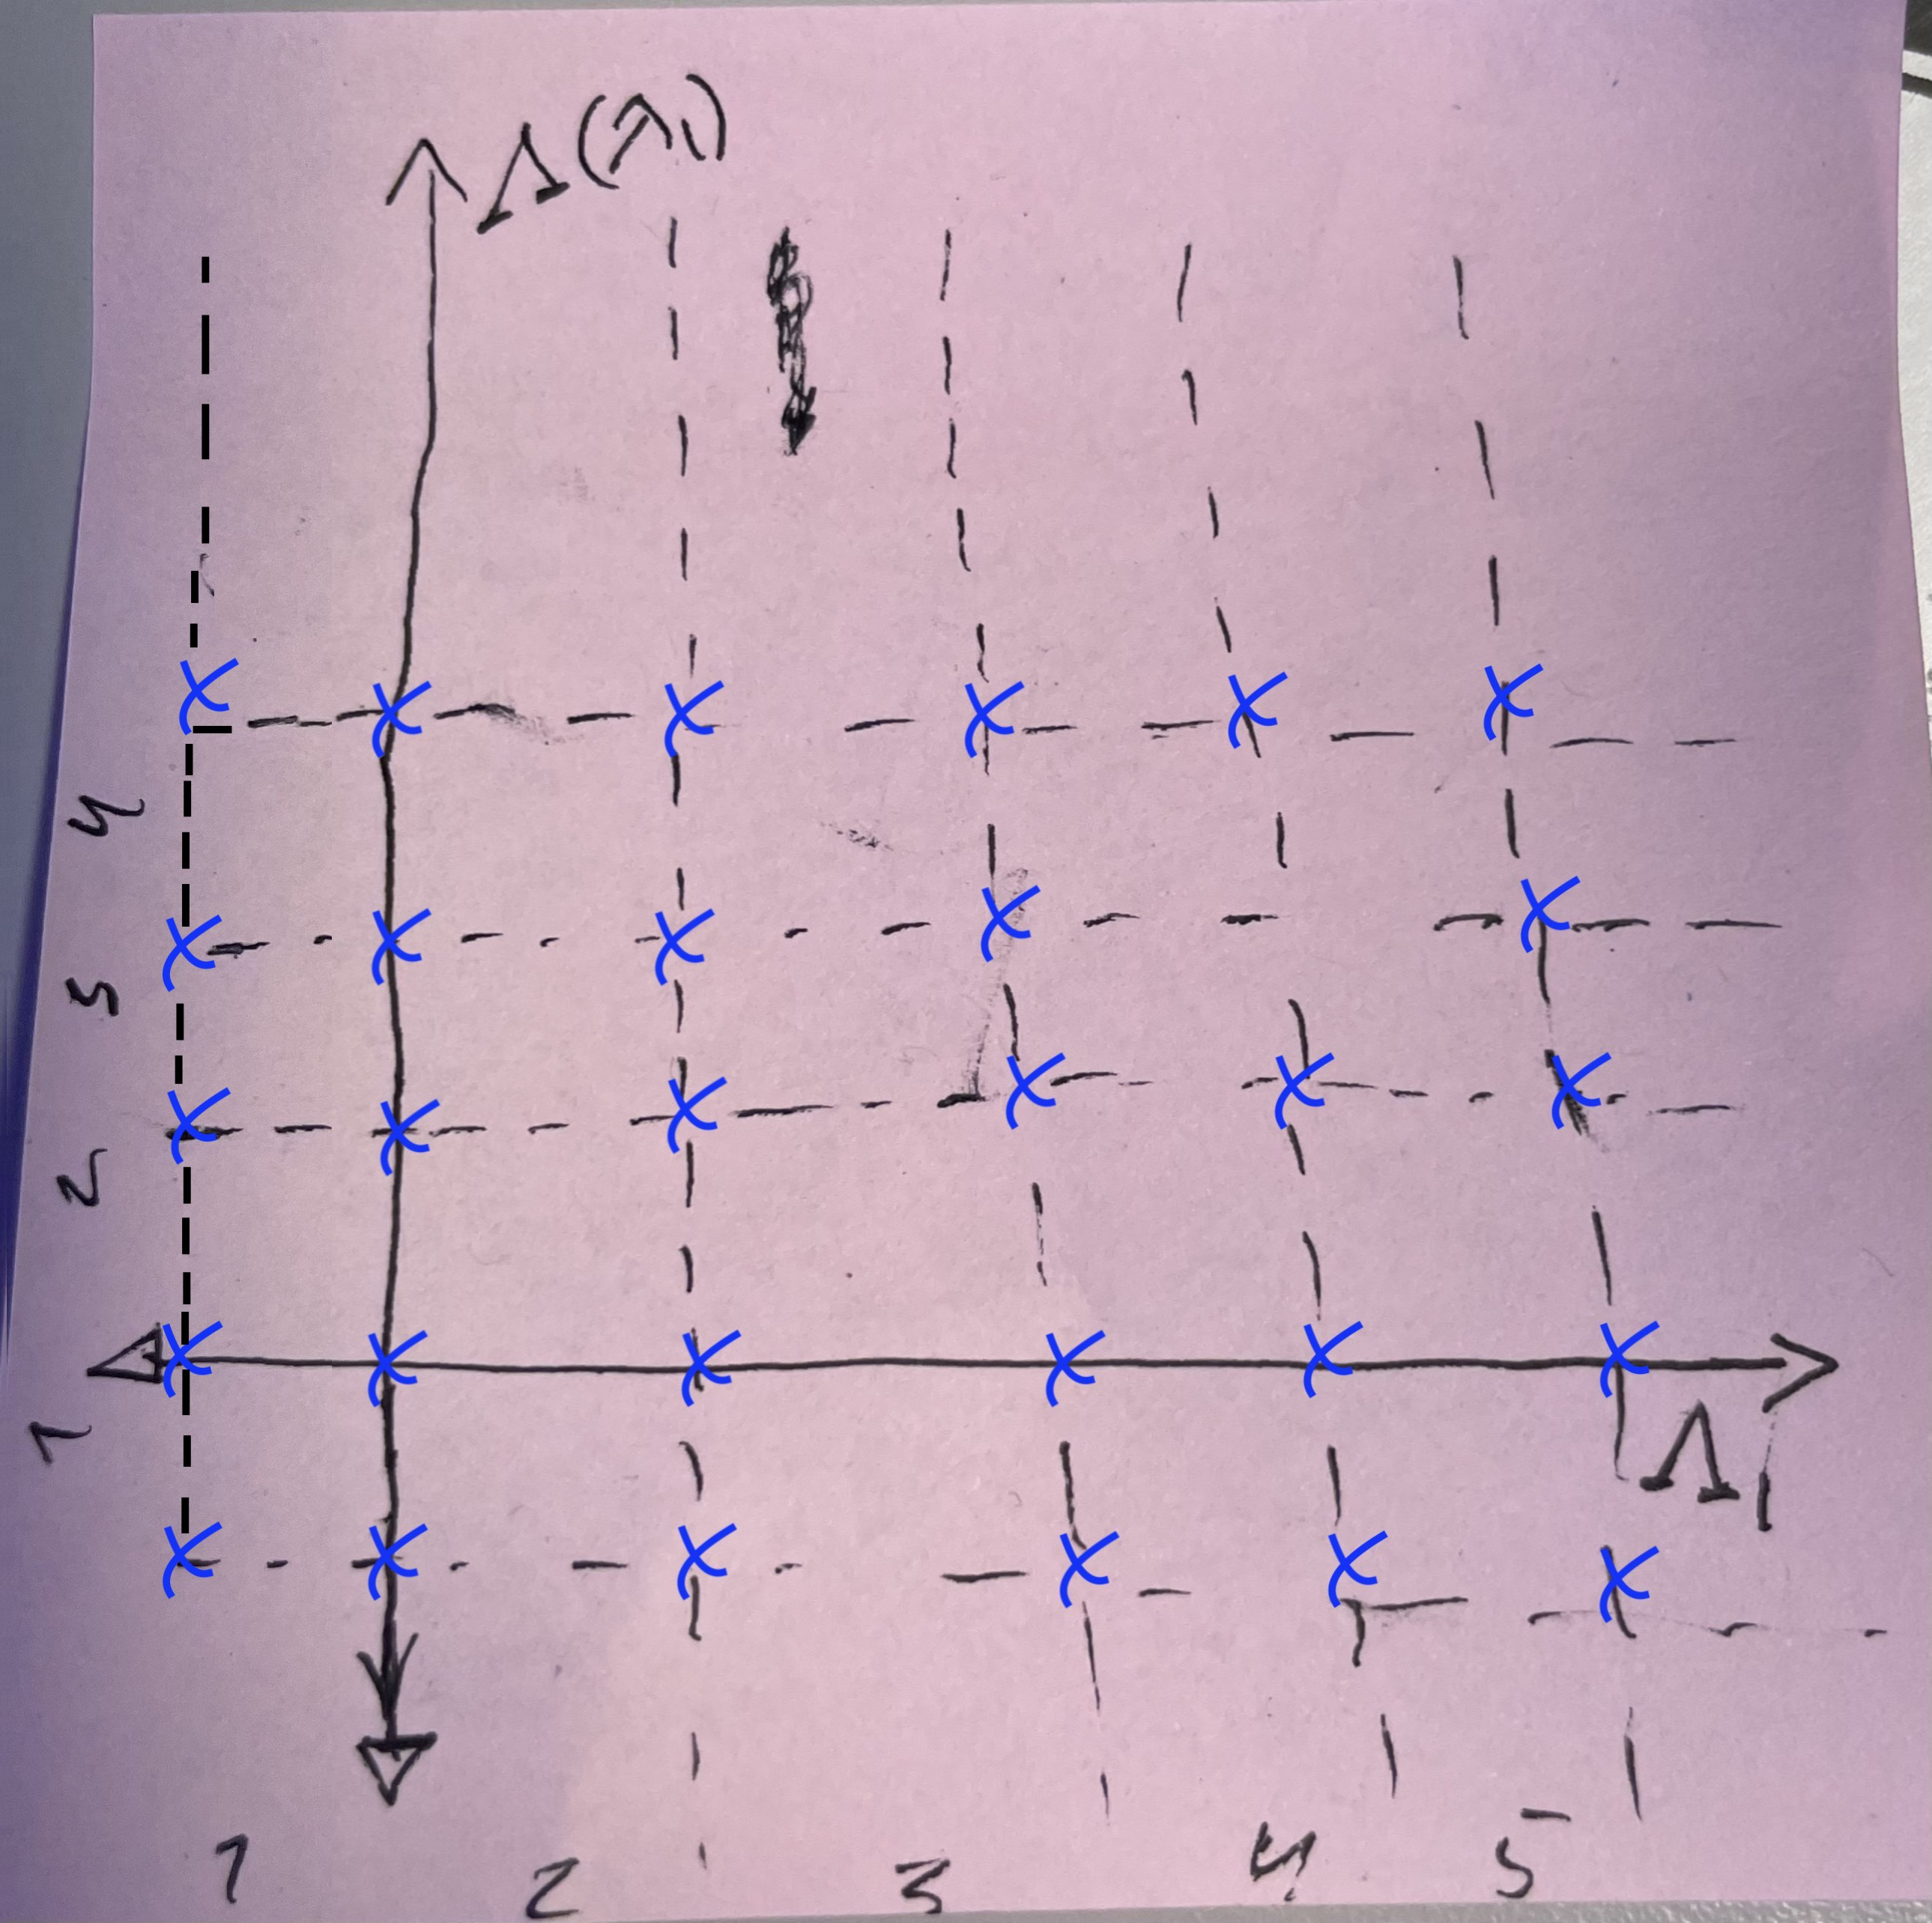
\includegraphics[width=0.9\linewidth]{spec_no_shift.jpg}
        %* Figure 1
        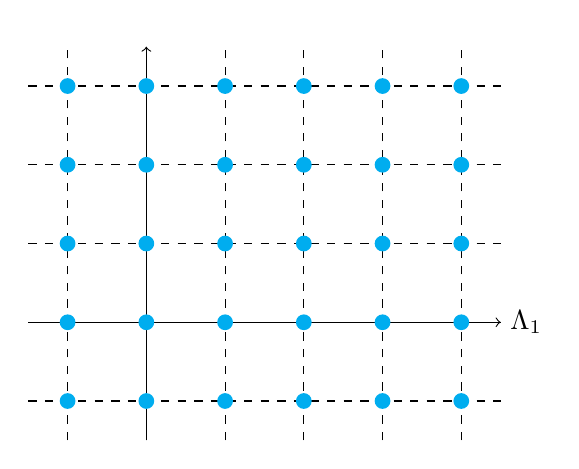
\begin{tikzpicture}
            \foreach \z in {0}{  % Controles whether the axes are inverted or not, 1 = yes, anything else = no
                

\ifnum\z=1
    % Axis lines
    %\draw[->] (-1.5,0) -- (4.5,0) node[above, xshift=2ex] {$\lambfuncGen{\lambda_2}$};
    \draw[->] (-1.5,0) -- (4.5,0) node[right] {$\lambfuncGen{\lambda_2}$};
    \draw[->] (0,-1.5) -- (0,3.5) node[above] {$\Lambda_2$};

    % Dashed lines at each integer in the x direction
    \foreach \x in {-1,...,4}
        \draw[dashed] (\x,-1.5) -- (\x,3.5);

    % Dashed lines at each integer in the y direction
    \foreach \y in {-1,...,3}
        \draw[dashed] (-1.5,\y) -- (4.5,\y);
\else
    % Axis lines
    \draw[->] (-1.5,0) -- (4.5,0) node[right] {$\Lambda_1$};
    \draw[->] (0,-1.5) -- (0,3.5) node[above] {$\lambfunc$};

    % Dashed lines at each integer in the x direction
    \foreach \x in {-1,...,4}
        \draw[dashed] (\x,-1.5) -- (\x,3.5);

    % Dashed lines at each integer in the y direction
    \foreach \y in {-1,...,3}
        \draw[dashed] (-1.5,\y) -- (4.5,\y);
\fi
                % Cyan circles at an integer coordinate with no border
                \foreach \x in {-1,...,4}
                    \foreach \y in {-1,...,3}
                        \fill[cyan] (\x,\y) circle (0.1);
            }
        \end{tikzpicture}
        %* —————————————————
        \caption{Lattice spectra}
        \label{fig:lattice_spectra}
    \end{subfigure}\quad
    \begin{subfigure}{.47\textwidth}
        \centering
        %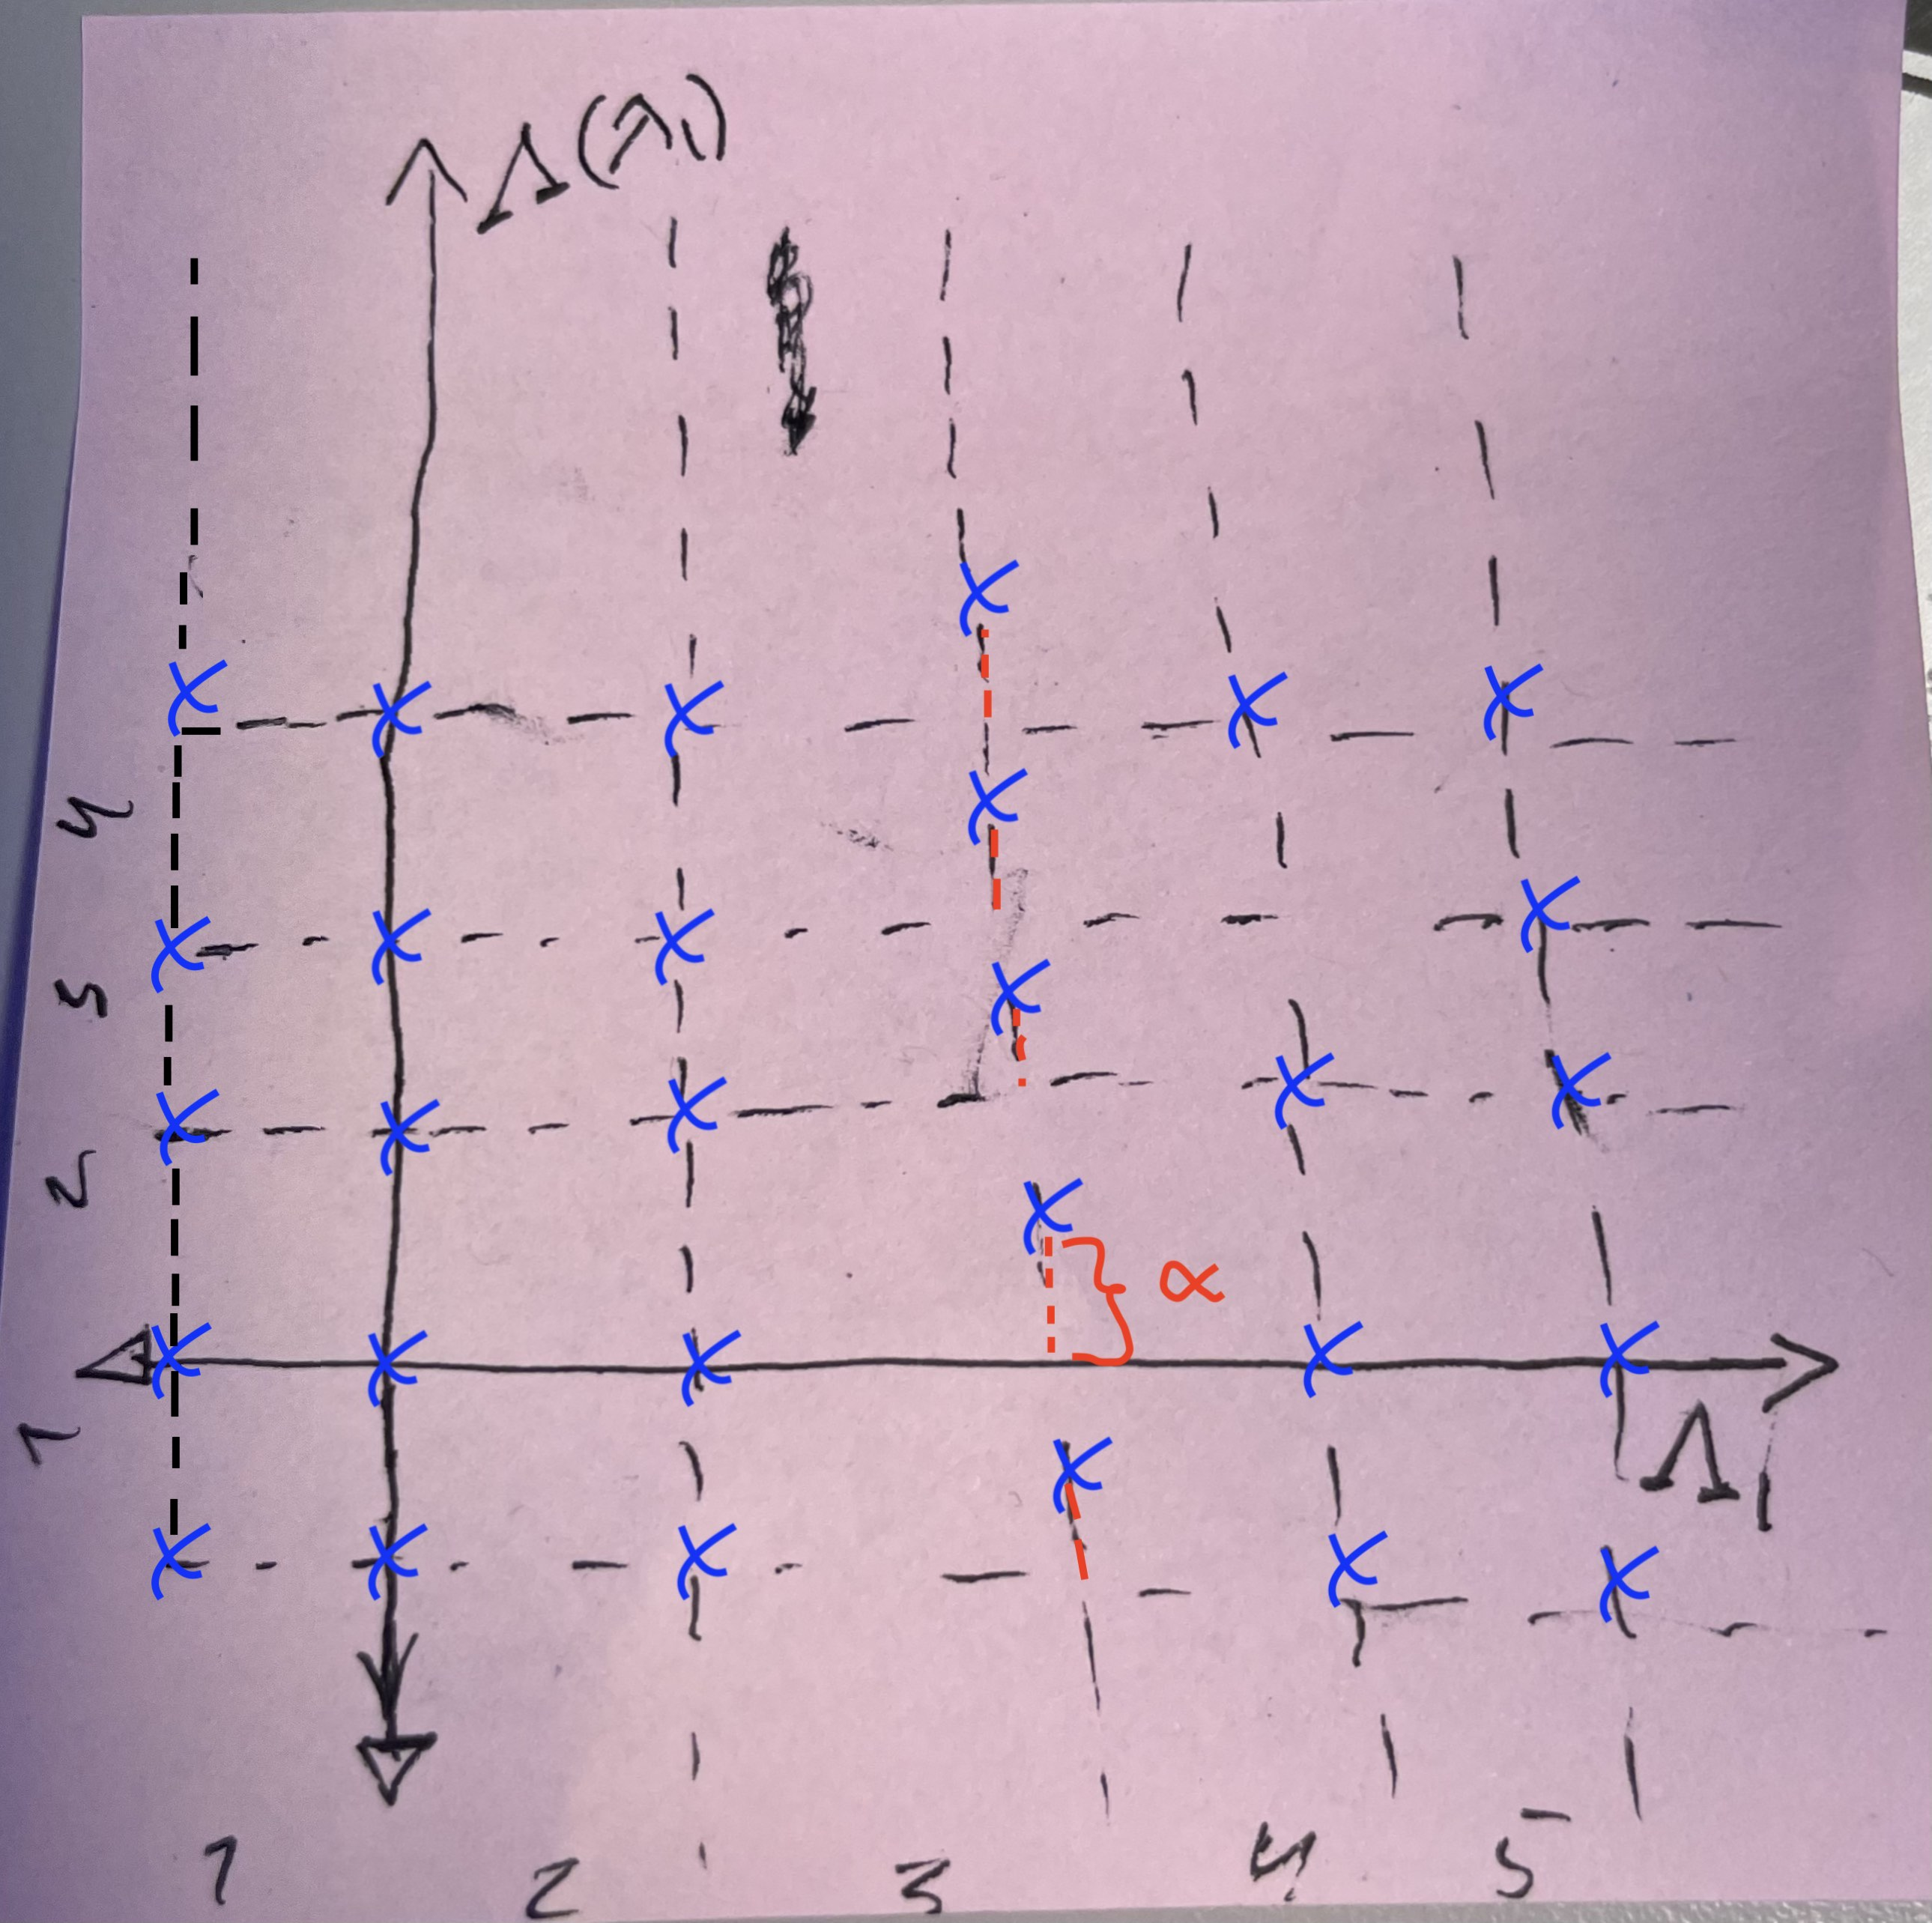
\includegraphics[width=0.9\linewidth]{spec_single_shift.jpg}
        %* Figure 2
        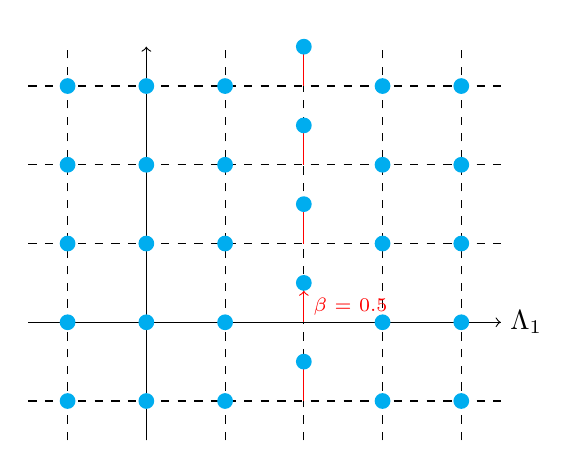
\begin{tikzpicture}
            \foreach \z in {0}{  % Controles whether the axes are inverted or not, 1 = yes, anything else = no
                

\ifnum\z=1
    % Axis lines
    %\draw[->] (-1.5,0) -- (4.5,0) node[above, xshift=2ex] {$\lambfuncGen{\lambda_2}$};
    \draw[->] (-1.5,0) -- (4.5,0) node[right] {$\lambfuncGen{\lambda_2}$};
    \draw[->] (0,-1.5) -- (0,3.5) node[above] {$\Lambda_2$};

    % Dashed lines at each integer in the x direction
    \foreach \x in {-1,...,4}
        \draw[dashed] (\x,-1.5) -- (\x,3.5);

    % Dashed lines at each integer in the y direction
    \foreach \y in {-1,...,3}
        \draw[dashed] (-1.5,\y) -- (4.5,\y);
\else
    % Axis lines
    \draw[->] (-1.5,0) -- (4.5,0) node[right] {$\Lambda_1$};
    \draw[->] (0,-1.5) -- (0,3.5) node[above] {$\lambfunc$};

    % Dashed lines at each integer in the x direction
    \foreach \x in {-1,...,4}
        \draw[dashed] (\x,-1.5) -- (\x,3.5);

    % Dashed lines at each integer in the y direction
    \foreach \y in {-1,...,3}
        \draw[dashed] (-1.5,\y) -- (4.5,\y);
\fi
                % The single shift 
                \def\BetaSingle{0.5}

                % x in the range [-1,1]
                % Cyan circles at an integer coordinate with no border
                \foreach \x in {-1,...,1}
                \foreach \y in {-1,...,3}
                    \fill[cyan] (\x,\y) circle (0.1);  % Cyan circle
                    %\draw[fill=cyan] (\x,\y) circle (0.1);  % Black circle with cyan fill

                % x = 2
                \foreach \x in {2}{
                \foreach \y in {-1,...,3}{
                    \ifnum\y=0
                        %\draw[->, thick, red] (\x,\y) -- (\x,\y+\BetaSingle-0.1) node[midway, right] {\scriptsize $\beta$ = \BetaSingle};  % Line indicating the shift amount
                        \draw[->, red] (\x,\y) -- (\x,\y+\BetaSingle-0.1) node[midway, right] {\scriptsize $\beta$ = \BetaSingle};  % Line indicating the shift amount
                    \else
                        \draw[red] (\x,\y) -- (\x,\y+\BetaSingle);  % Line indicating the shift amount
                    \fi
                    \fill[cyan] (\x,\y+\BetaSingle) circle (0.1);  % Cyan circles at an integer coordinate with no border
                    %\draw[fill=cyan] (\x,\y+\BetaSingle) circle (0.1);  % Black circle with cyan fill
                }}

                % x in the range [3,4]
                % Cyan circles at an integer coordinate with no border
                \foreach \x in {3,...,4}{
                    \foreach \y in {-1,...,3}{
                        \fill[cyan] (\x,\y) circle (0.1);  % Cyan circle
                        %\draw[fill=cyan] (\x,\y) circle (0.1);  % Black circle with cyan fill
                }}
            }
        \end{tikzpicture}
        %* —————————————————
        \caption{Single vertical shift}
        \label{fig:single_shift_vertical}
    \end{subfigure}\\
    \begin{subfigure}{.47\textwidth}
        \centering
        %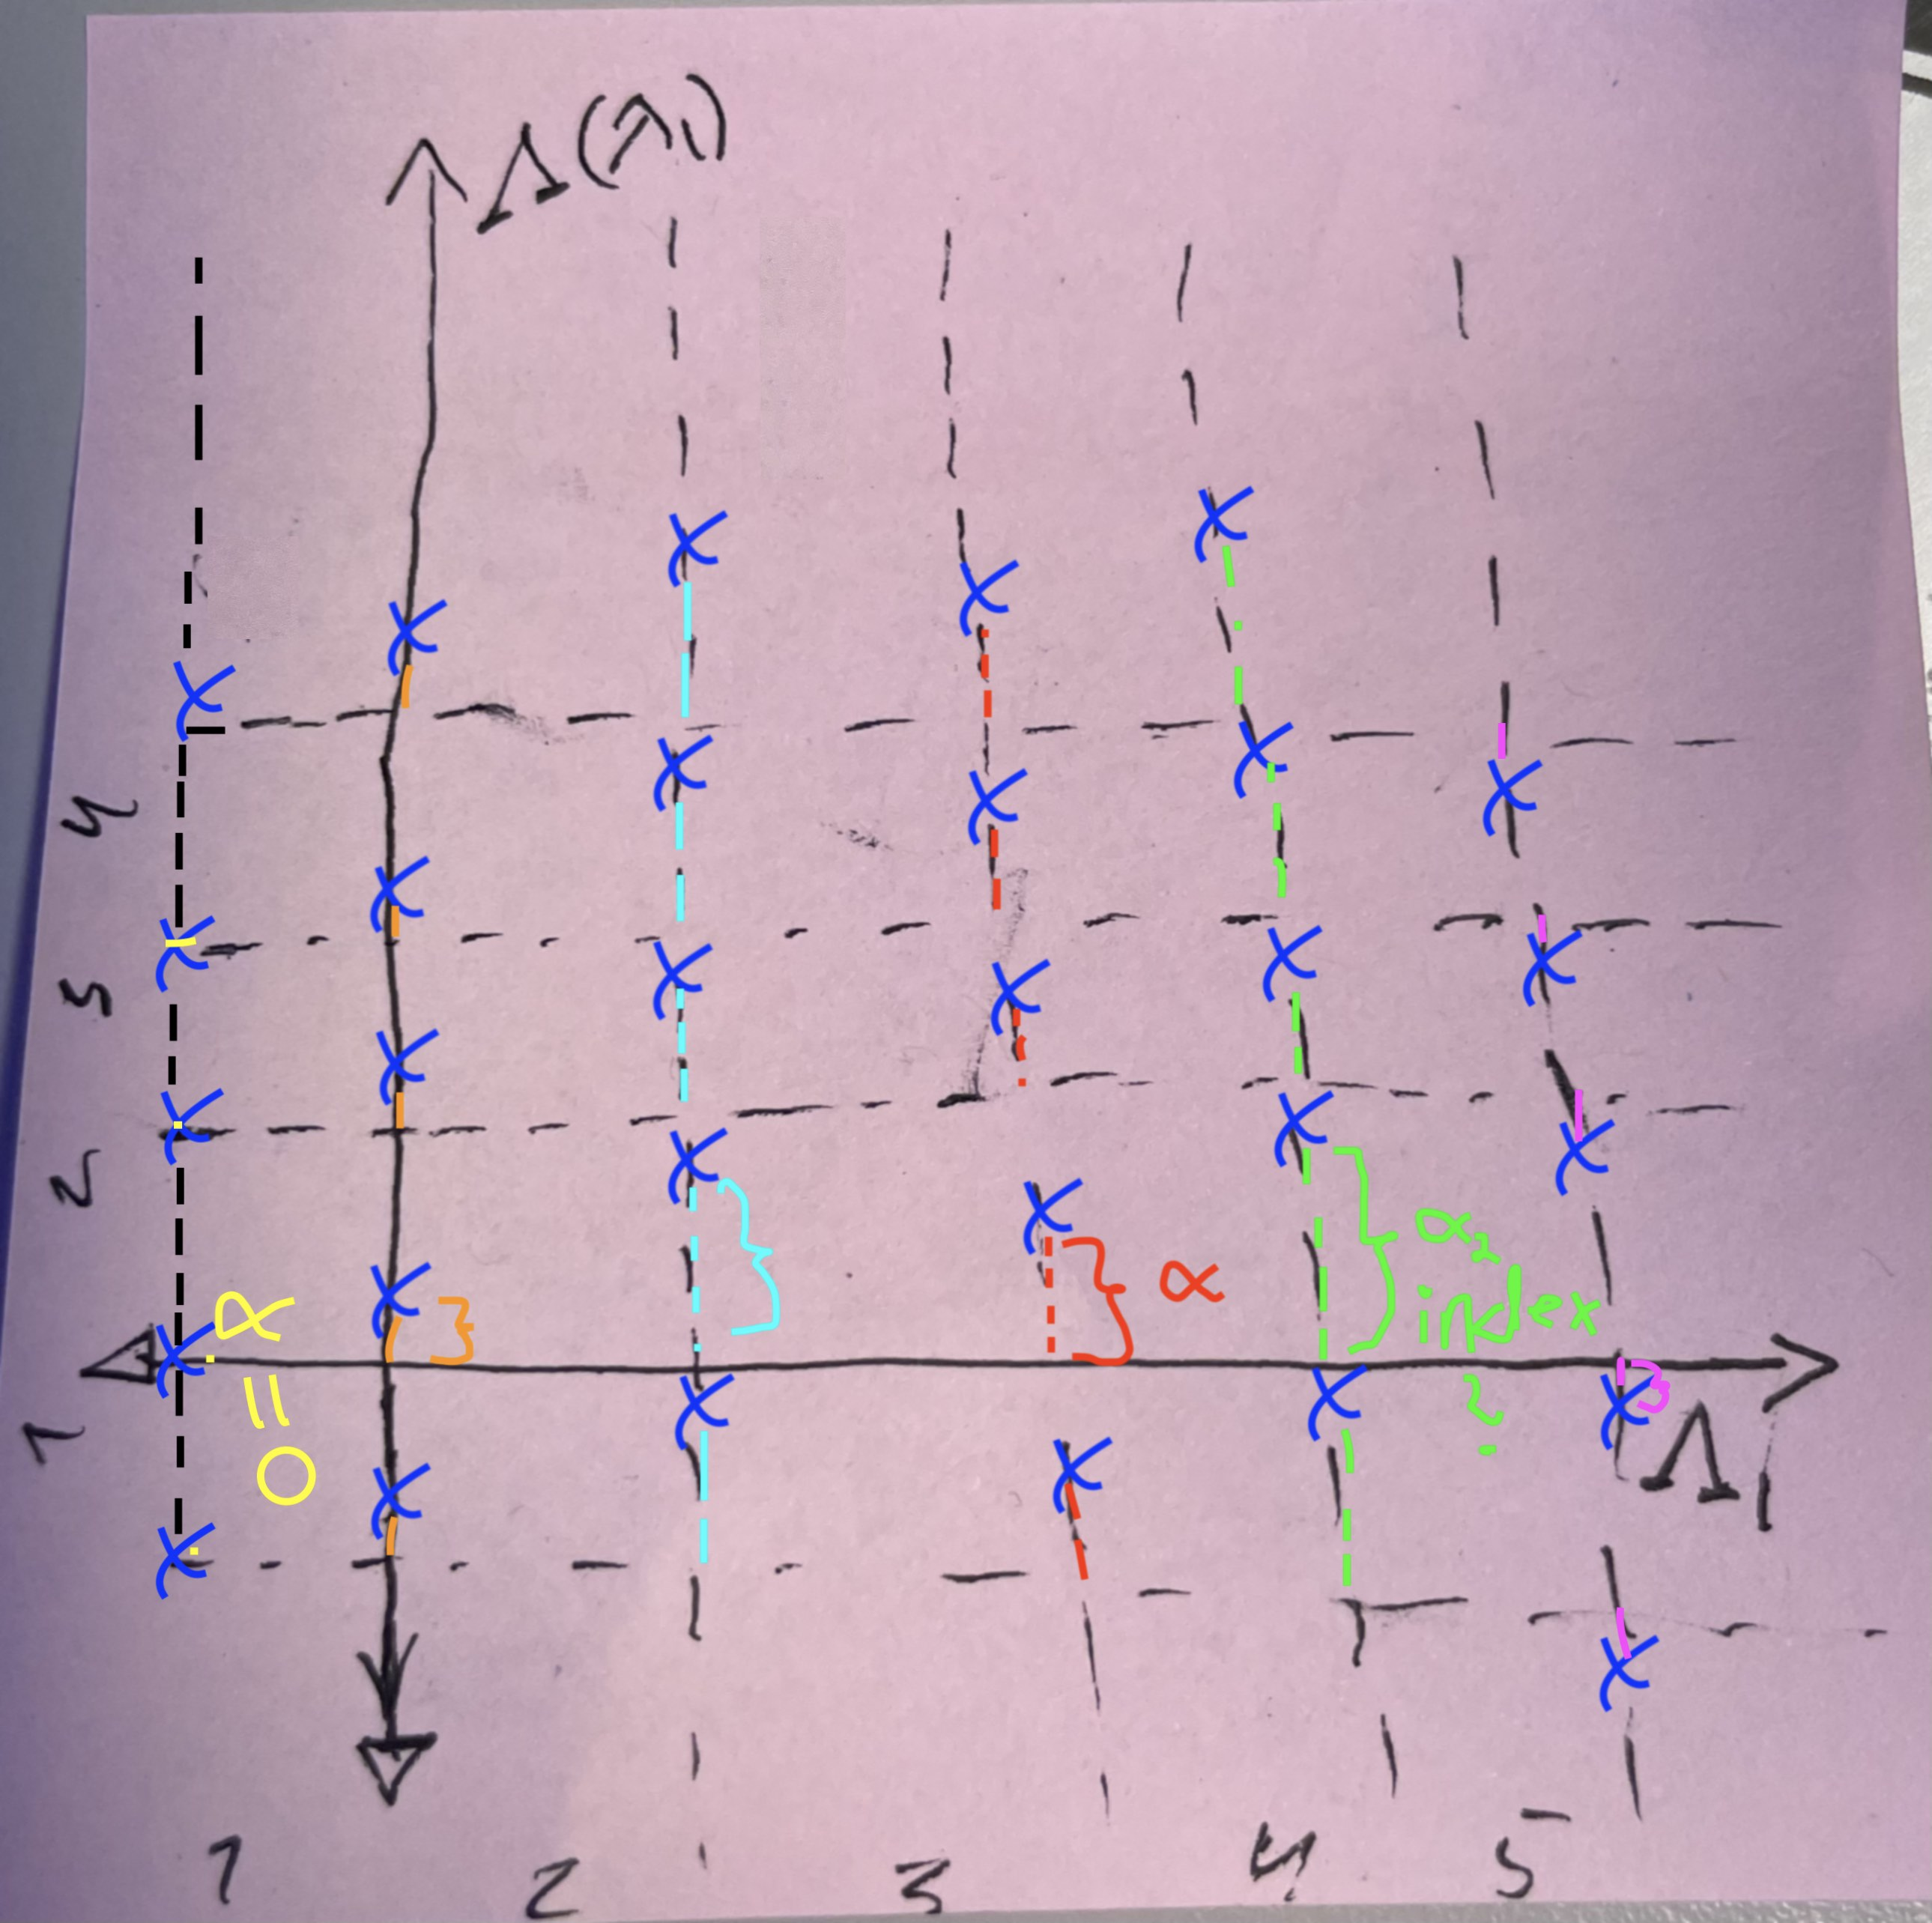
\includegraphics[width=0.9\linewidth]{multiple_shift_left_zero.jpg}
        %* Figure 3
        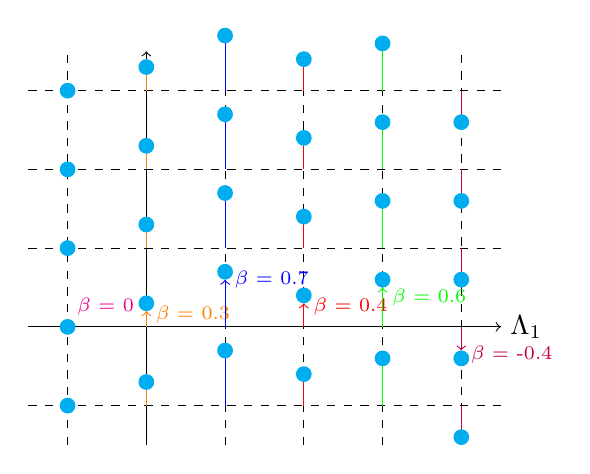
\begin{tikzpicture}
            \foreach \z in {0}{  % Controles whether the axes are inverted or not, 1 = yes, anything else = no
                

\ifnum\z=1
    % Axis lines
    %\draw[->] (-1.5,0) -- (4.5,0) node[above, xshift=2ex] {$\lambfuncGen{\lambda_2}$};
    \draw[->] (-1.5,0) -- (4.5,0) node[right] {$\lambfuncGen{\lambda_2}$};
    \draw[->] (0,-1.5) -- (0,3.5) node[above] {$\Lambda_2$};

    % Dashed lines at each integer in the x direction
    \foreach \x in {-1,...,4}
        \draw[dashed] (\x,-1.5) -- (\x,3.5);

    % Dashed lines at each integer in the y direction
    \foreach \y in {-1,...,3}
        \draw[dashed] (-1.5,\y) -- (4.5,\y);
\else
    % Axis lines
    \draw[->] (-1.5,0) -- (4.5,0) node[right] {$\Lambda_1$};
    \draw[->] (0,-1.5) -- (0,3.5) node[above] {$\lambfunc$};

    % Dashed lines at each integer in the x direction
    \foreach \x in {-1,...,4}
        \draw[dashed] (\x,-1.5) -- (\x,3.5);

    % Dashed lines at each integer in the y direction
    \foreach \y in {-1,...,3}
        \draw[dashed] (-1.5,\y) -- (4.5,\y);
\fi
                % Shift list
                \def\BetaMinOne{0}
                \def\BetaZero{0.3}
                \def\BetaOne{0.7}
                \def\BetaTwo{0.4}
                \def\BetaThree{0.6}
                \def\BetaFour{-0.4}

                % x = -1
                \foreach \x in {-1}{
                \foreach \y in {-1,...,3}{
                    \ifnum\y=0
                    \draw[->, magenta] (\x,\y) -- (\x,\y+0.05\BetaMinOne) node[midway, above right] {\scriptsize $\beta$ = \BetaMinOne};  % Line indicating the shift amount
                    \else
                    \draw[magenta] (\x,\y) -- (\x,\y+\BetaMinOne);  % Line indicating the shift amount
                    \fi
                    \fill[cyan] (\x,\y+\BetaMinOne) circle (0.1);  % Cyan circles at an integer coordinate with no border
                }}
                % x = 0
                \foreach \x in {0}{
                \foreach \y in {-1,...,3}{
                    \ifnum\y=0
                    \draw[->, orange] (\x,\y) -- (\x,\y+\BetaZero-0.1) node[near end, right] {\scriptsize $\beta$ = \BetaZero};  % Line indicating the shift amount
                    \else
                    \draw[orange] (\x,\y) -- (\x,\y+\BetaZero);  % Line indicating the shift amount
                    \fi
                    \fill[cyan] (\x,\y+\BetaZero) circle (0.1);  % Cyan circles at an integer coordinate with no border
                }}
                % x = 1
                \foreach \x in {1}{
                \foreach \y in {-1,...,3}{
                    \ifnum\y=0
                    \draw[->, blue] (\x,\y) -- (\x,\y+\BetaOne-0.1) node[at end, right] {\scriptsize $\beta$ = \BetaOne};  % Line indicating the shift amount
                    \else
                    \draw[blue] (\x,\y) -- (\x,\y+\BetaOne);  % Line indicating the shift amount
                    \fi
                    \fill[cyan] (\x,\y+\BetaOne) circle (0.1);  % Cyan circles at an integer coordinate with no border
                }}
                % x = 2
                \foreach \x in {2}{
                \foreach \y in {-1,...,3}{
                    \ifnum\y=0
                    \draw[->, red] (\x,\y) -- (\x,\y+\BetaTwo-0.1) node[very near end, right] {\scriptsize $\beta$ = \BetaTwo};  % Line indicating the shift amount
                    \else
                    \draw[red] (\x,\y) -- (\x,\y+\BetaTwo);  % Line indicating the shift amount
                    \fi
                    \fill[cyan] (\x,\y+\BetaTwo) circle (0.1);  % Cyan circles at an integer coordinate with no border
                }}
                % x = 3
                \foreach \x in {3}{
                \foreach \y in {-1,...,3}{
                    \ifnum\y=0
                    \draw[->, green] (\x,\y) -- (\x,\y+\BetaThree-0.1) node[near end, right] {\scriptsize $\beta$ = \BetaThree};  % Line indicating the shift amount
                    \else
                    \draw[green] (\x,\y) -- (\x,\y+\BetaThree);  % Line indicating the shift amount
                    \fi
                    \fill[cyan] (\x,\y+\BetaThree) circle (0.1);  % Cyan circles at an integer coordinate with no border
                }}
                % x = 4
                \foreach \x in {4}{
                \foreach \y in {-1,...,3}{
                    \ifnum\y=0
                    \draw[->, purple] (\x,\y) -- (\x,\y+\BetaFour+0.1) node[at end, right, yshift=-0.5mm] {\scriptsize $\beta$ = \BetaFour};  % Line indicating the shift amount
                    \else
                    \draw[purple] (\x,\y) -- (\x,\y+\BetaFour);  % Line indicating the shift amount
                    \fi
                    \fill[cyan] (\x,\y+\BetaFour) circle (0.1);  % Cyan circles at an integer coordinate with no border
                }}
            }
        \end{tikzpicture}
        %* —————————————————
        \caption{Multiple individual vertical shifts}
        \label{fig:multiple_shift_vertical}
    \end{subfigure}\quad
    \begin{subfigure}{.47\textwidth}
        \centering
        %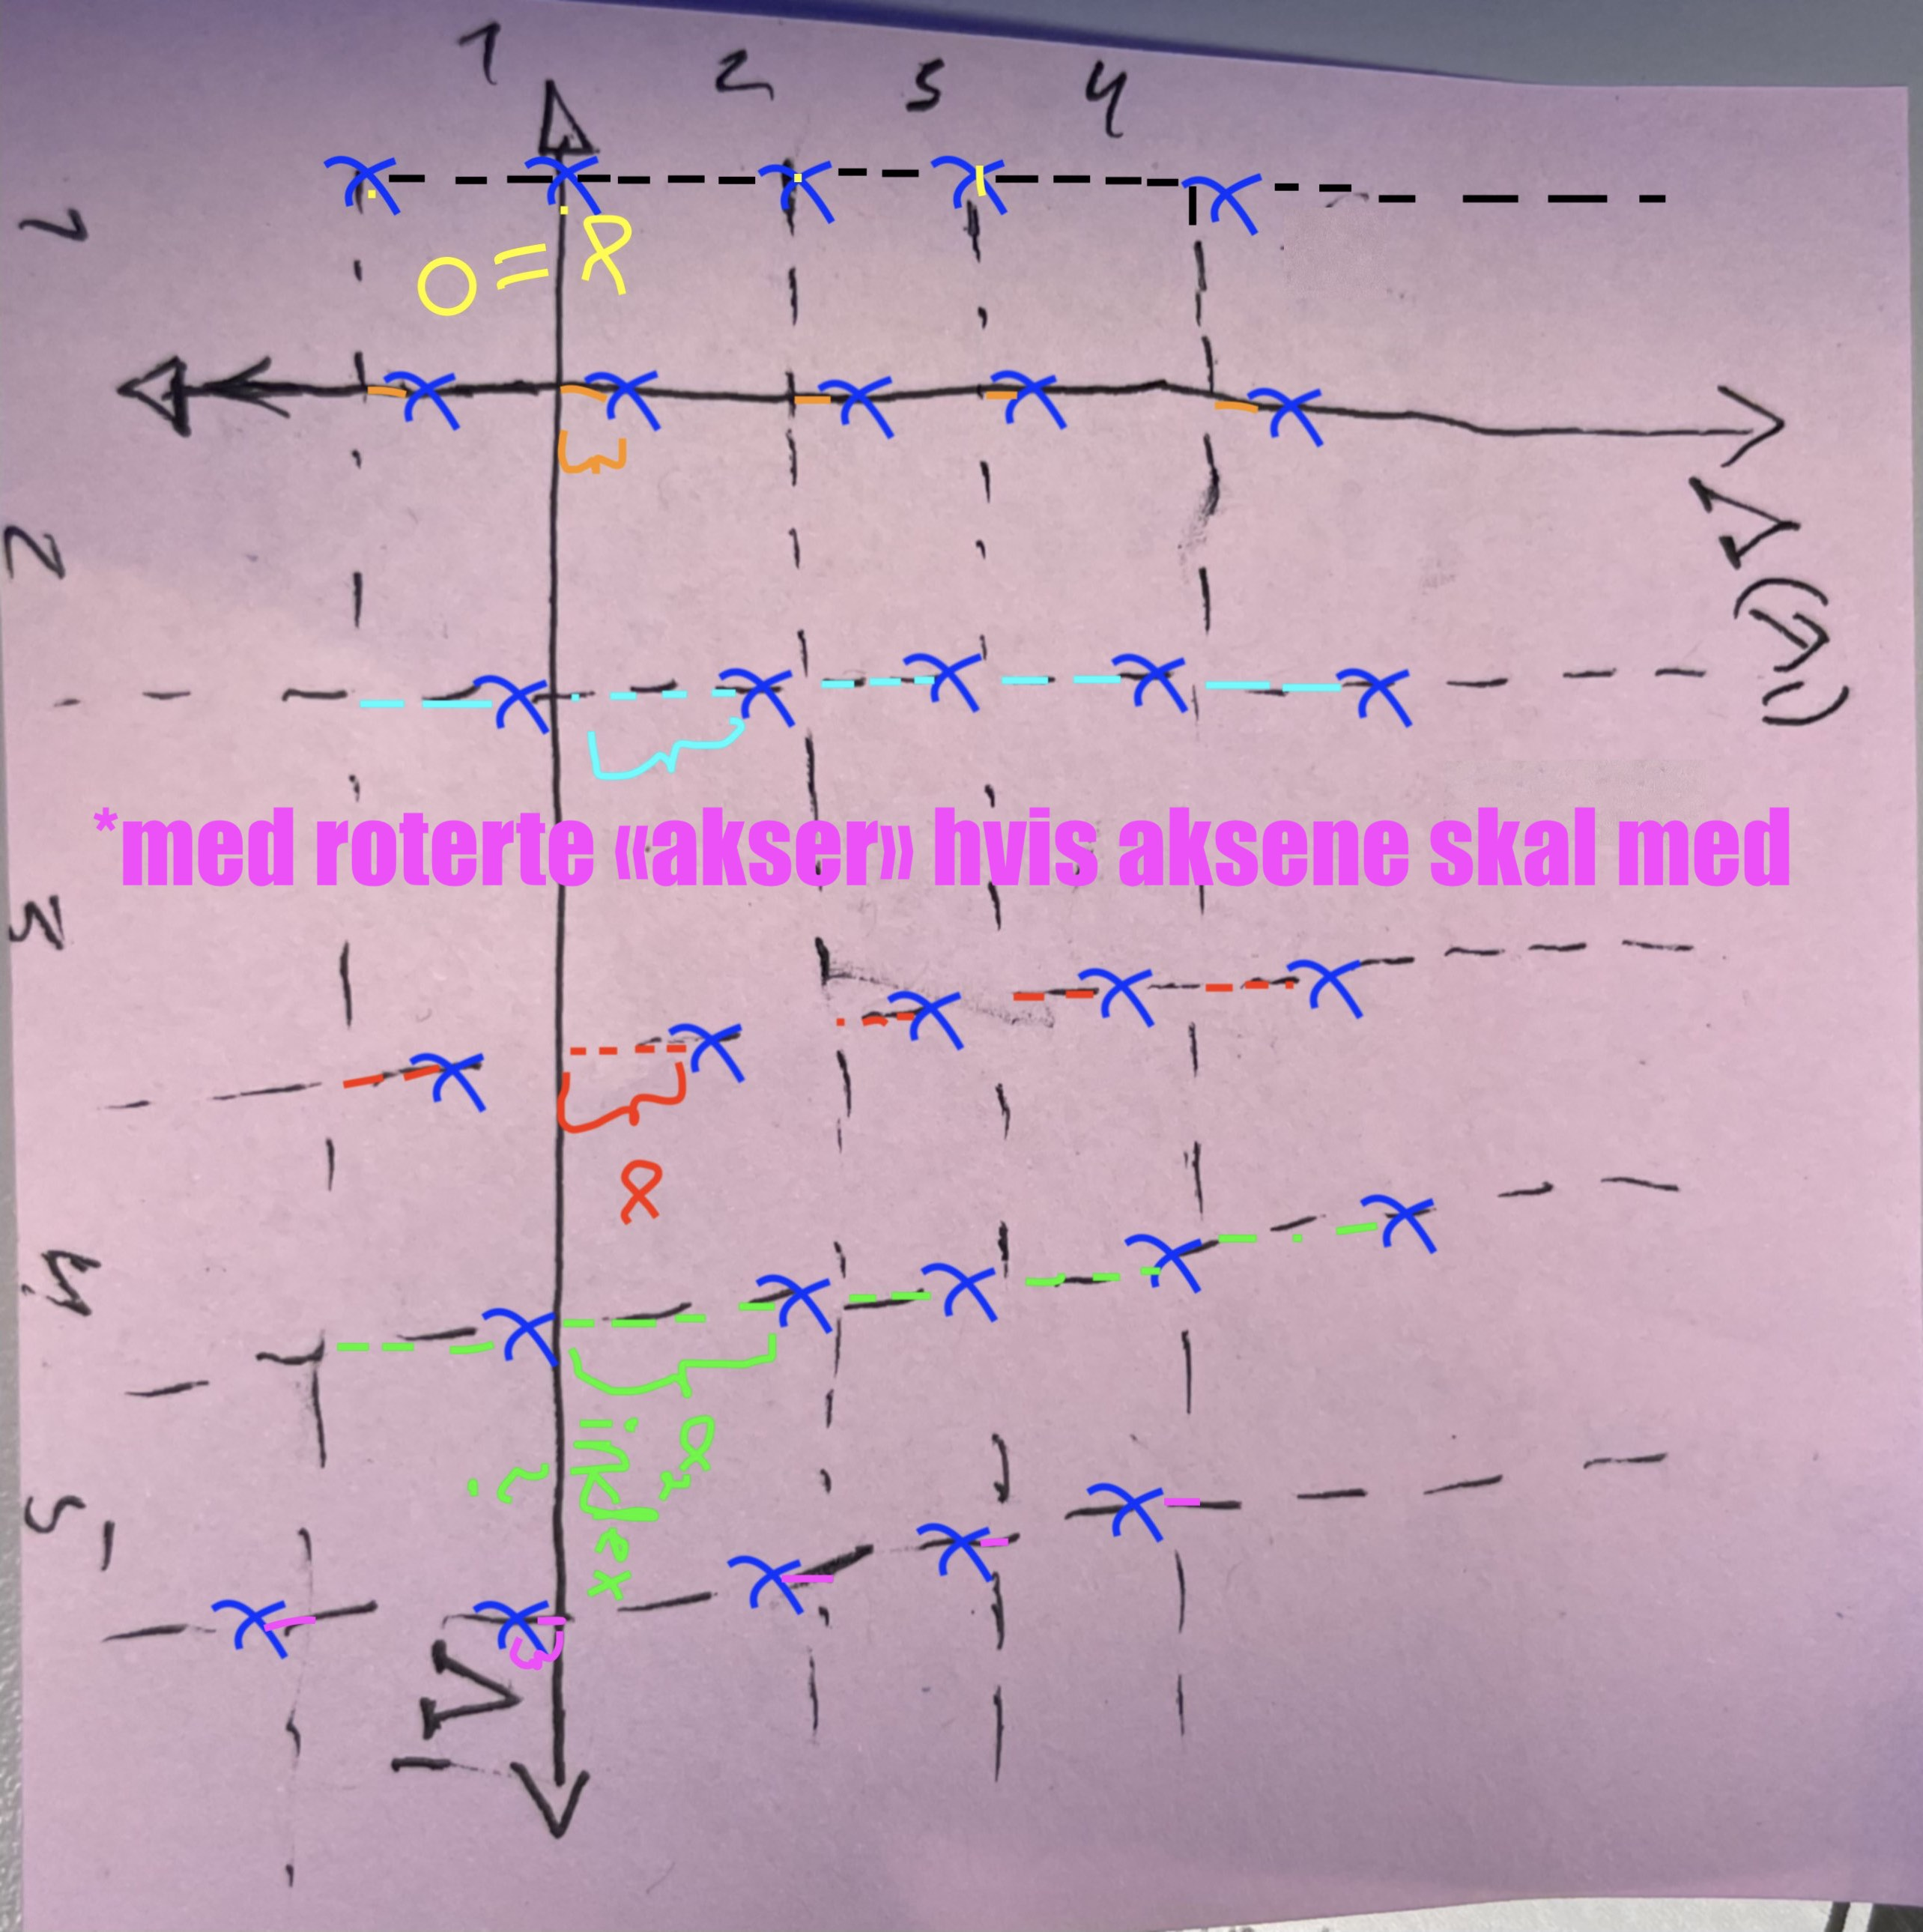
\includegraphics[width=0.9\linewidth]{multiple_shift_left_zero_horizontal.jpg}
        %* Figure 4
        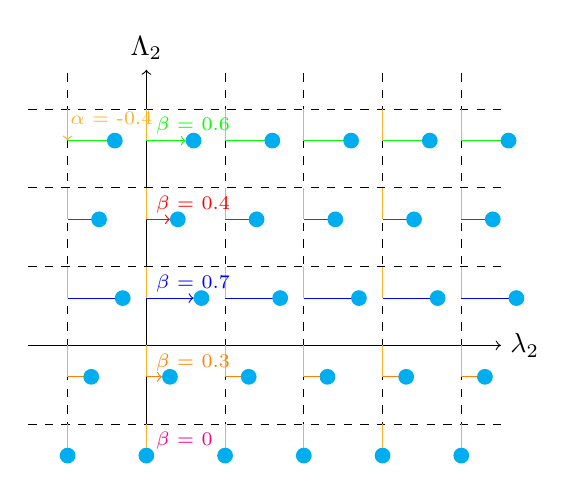
\begin{tikzpicture}
            \foreach \z in {1}{  % Controles whether the axes are inverted or not, 1 = yes, anything else = no
                

\ifnum\z=1
    % Axis lines
    %\draw[->] (-1.5,0) -- (4.5,0) node[above, xshift=2ex] {$\lambfuncGen{\lambda_2}$};
    \draw[->] (-1.5,0) -- (4.5,0) node[right] {$\lambfuncGen{\lambda_2}$};
    \draw[->] (0,-1.5) -- (0,3.5) node[above] {$\Lambda_2$};

    % Dashed lines at each integer in the x direction
    \foreach \x in {-1,...,4}
        \draw[dashed] (\x,-1.5) -- (\x,3.5);

    % Dashed lines at each integer in the y direction
    \foreach \y in {-1,...,3}
        \draw[dashed] (-1.5,\y) -- (4.5,\y);
\else
    % Axis lines
    \draw[->] (-1.5,0) -- (4.5,0) node[right] {$\Lambda_1$};
    \draw[->] (0,-1.5) -- (0,3.5) node[above] {$\lambfunc$};

    % Dashed lines at each integer in the x direction
    \foreach \x in {-1,...,4}
        \draw[dashed] (\x,-1.5) -- (\x,3.5);

    % Dashed lines at each integer in the y direction
    \foreach \y in {-1,...,3}
        \draw[dashed] (-1.5,\y) -- (4.5,\y);
\fi
                % Shift list
                \def\BetaMinOne{0}
                \def\BetaZero{0.3}
                \def\BetaOne{0.7}
                \def\BetaTwo{0.4}
                \def\BetaThree{0.6}
                \def\BetaFour{-0.6}
                \def\AlphaONE{-0.4}

                % The X shift lines at x=0
                \foreach \x in {-1,...,4}{
                \foreach \y in {-1,...,3}{
                    \ifnum\x=-1
                        \ifnum\y=3
                            \draw[->, Dandelion] (\x,\y) -- (\x,\y+\AlphaONE) node[pos=0.3, right, xshift=-0.9mm] {\scriptsize $\alpha$ = \AlphaONE};  % Line indicating the shift amount
                        \else
                            %\draw[->, thick, purple] (\x,\y) -- (\x,\y+\AlphaONE);  % Line indicating the shift amount
                            \draw[Dandelion] (\x,\y) -- (\x,\y+\AlphaONE);  % Line indicating the shift amount
                        \fi
                    \else
                    \draw[Dandelion] (\x,\y) -- (\x,\y+\AlphaONE);  % Line indicating the shift amount
                    \fi
                }}

                % The Y shift
                % y = -1
                \foreach \y in {-1}{
                \foreach \x in {-1,...,4}{
                    \ifnum\x=0
                    \draw[->, magenta] (\x,\y+\AlphaONE) -- (\x+\BetaMinOne+0.05, \y+\AlphaONE) node[at start, above right, yshift=-0.5mm] {\scriptsize $\beta$ = \BetaMinOne};  % Line indicating the shift amount
                    \else
                    \draw[magenta] (\x,\y+\AlphaONE) -- (\x+\BetaMinOne,\y+\AlphaONE);  % Line indicating the shift amount
                    \fi
                    \fill[cyan] (\x+\BetaMinOne,\y+\AlphaONE) circle (0.1);  % Cyan circles at an integer coordinate with no border
                }}
                % y = 0
                \foreach \y in {0}{
                \foreach \x in {-1,...,4}{
                    \ifnum\x=0
                    \draw[->, orange] (\x,\y+\AlphaONE) -- (\x+\BetaZero-0.1,\y+\AlphaONE) node[at start, above right, yshift=-0.5mm] {\scriptsize $\beta$ = \BetaZero};  % Line indicating the shift amount
                    \else
                    \draw[orange] (\x,\y+\AlphaONE) -- (\x+\BetaZero,\y+\AlphaONE);  % Line indicating the shift amount
                    \fi
                    \fill[cyan] (\x+\BetaZero,\y+\AlphaONE) circle (0.1);  % Cyan circles at an integer coordinate with no border
                }}
                % y = 1
                \foreach \y in {1}{
                \foreach \x in {-1,...,4}{
                    \ifnum\x=0
                    \draw[->, blue] (\x,\y+\AlphaONE) -- (\x+\BetaOne-0.1,\y+\AlphaONE) node[at start, above right, yshift=-0.5mm] {\scriptsize $\beta$ = \BetaOne};  % Line indicating the shift amount
                    \else
                    \draw[blue] (\x,\y+\AlphaONE) -- (\x+\BetaOne,\y+\AlphaONE);  % Line indicating the shift amount
                    \fi
                    \fill[cyan] (\x+\BetaOne,\y+\AlphaONE) circle (0.1);  % Cyan circles at an integer coordinate with no border
                }}
                % y = 2
                \foreach \y in {2}{
                \foreach \x in {-1,...,4}{
                    \ifnum\x=0
                    \draw[->, red] (\x,\y+\AlphaONE) -- (\x+\BetaTwo-0.1,\y+\AlphaONE) node[at start, above right, yshift=-0.5mm] {\scriptsize $\beta$ = \BetaTwo};  % Line indicating the shift amount
                    \else
                    \draw[red] (\x,\y+\AlphaONE) -- (\x+\BetaTwo,\y+\AlphaONE);  % Line indicating the shift amount
                    \fi
                    \fill[cyan] (\x+\BetaTwo,\y+\AlphaONE) circle (0.1);  % Cyan circles at an integer coordinate with no border
                }}
                % y = 3
                \foreach \y in {3}{
                \foreach \x in {-1,...,4}{
                    \ifnum\x=0
                    \draw[->, green] (\x,\y+\AlphaONE) -- (\x+\BetaThree-0.1,\y+\AlphaONE) node[at start, above right, yshift=-0.5mm] {\scriptsize $\beta$ = \BetaThree};  % Line indicating the shift amount
                    \else
                    \draw[green] (\x,\y+\AlphaONE) -- (\x+\BetaThree,\y+\AlphaONE);  % Line indicating the shift amount
                    \fi
                    \fill[cyan] (\x+\BetaThree,\y+\AlphaONE) circle (0.1);  % Cyan circles at an integer coordinate with no border
                }}
            }
        \end{tikzpicture}
        %* —————————————————
        \caption{Multiple individual horizontal shifts}
        \label{fig:multiple_shift_horizontal}
    \end{subfigure}
    \label{fig:spectra_figures}
    \caption{Illustration of four spectral pairs for $(I^2,\Lambda)$ on a coordinate plane $X\times Y$. Dashed lines highlight the coordinate plane itself, and the cyan circles represent elements from the spectrum. In \cref{fig:lattice_spectra,fig:single_shift_vertical} $\Lambda$ is given by \labelcref{eq:first_construction} and \labelcref{eq:lam_single_shift_vertical} respectivly, where $\beta=0.5$ for the latter. In \cref{fig:multiple_shift_vertical,fig:multiple_shift_horizontal} $\Lambda$ is given by \labelcref{eq:lam_multiple_shift_vertical,eq:lam_multiple_shift_horizontal} respectivly.}
\end{figure}






\mycomment{  %! Block comment, thick lines in this figure

\begin{figure}[t]%h!
    \centering
    \begin{subfigure}{.47\textwidth}
        \centering
        %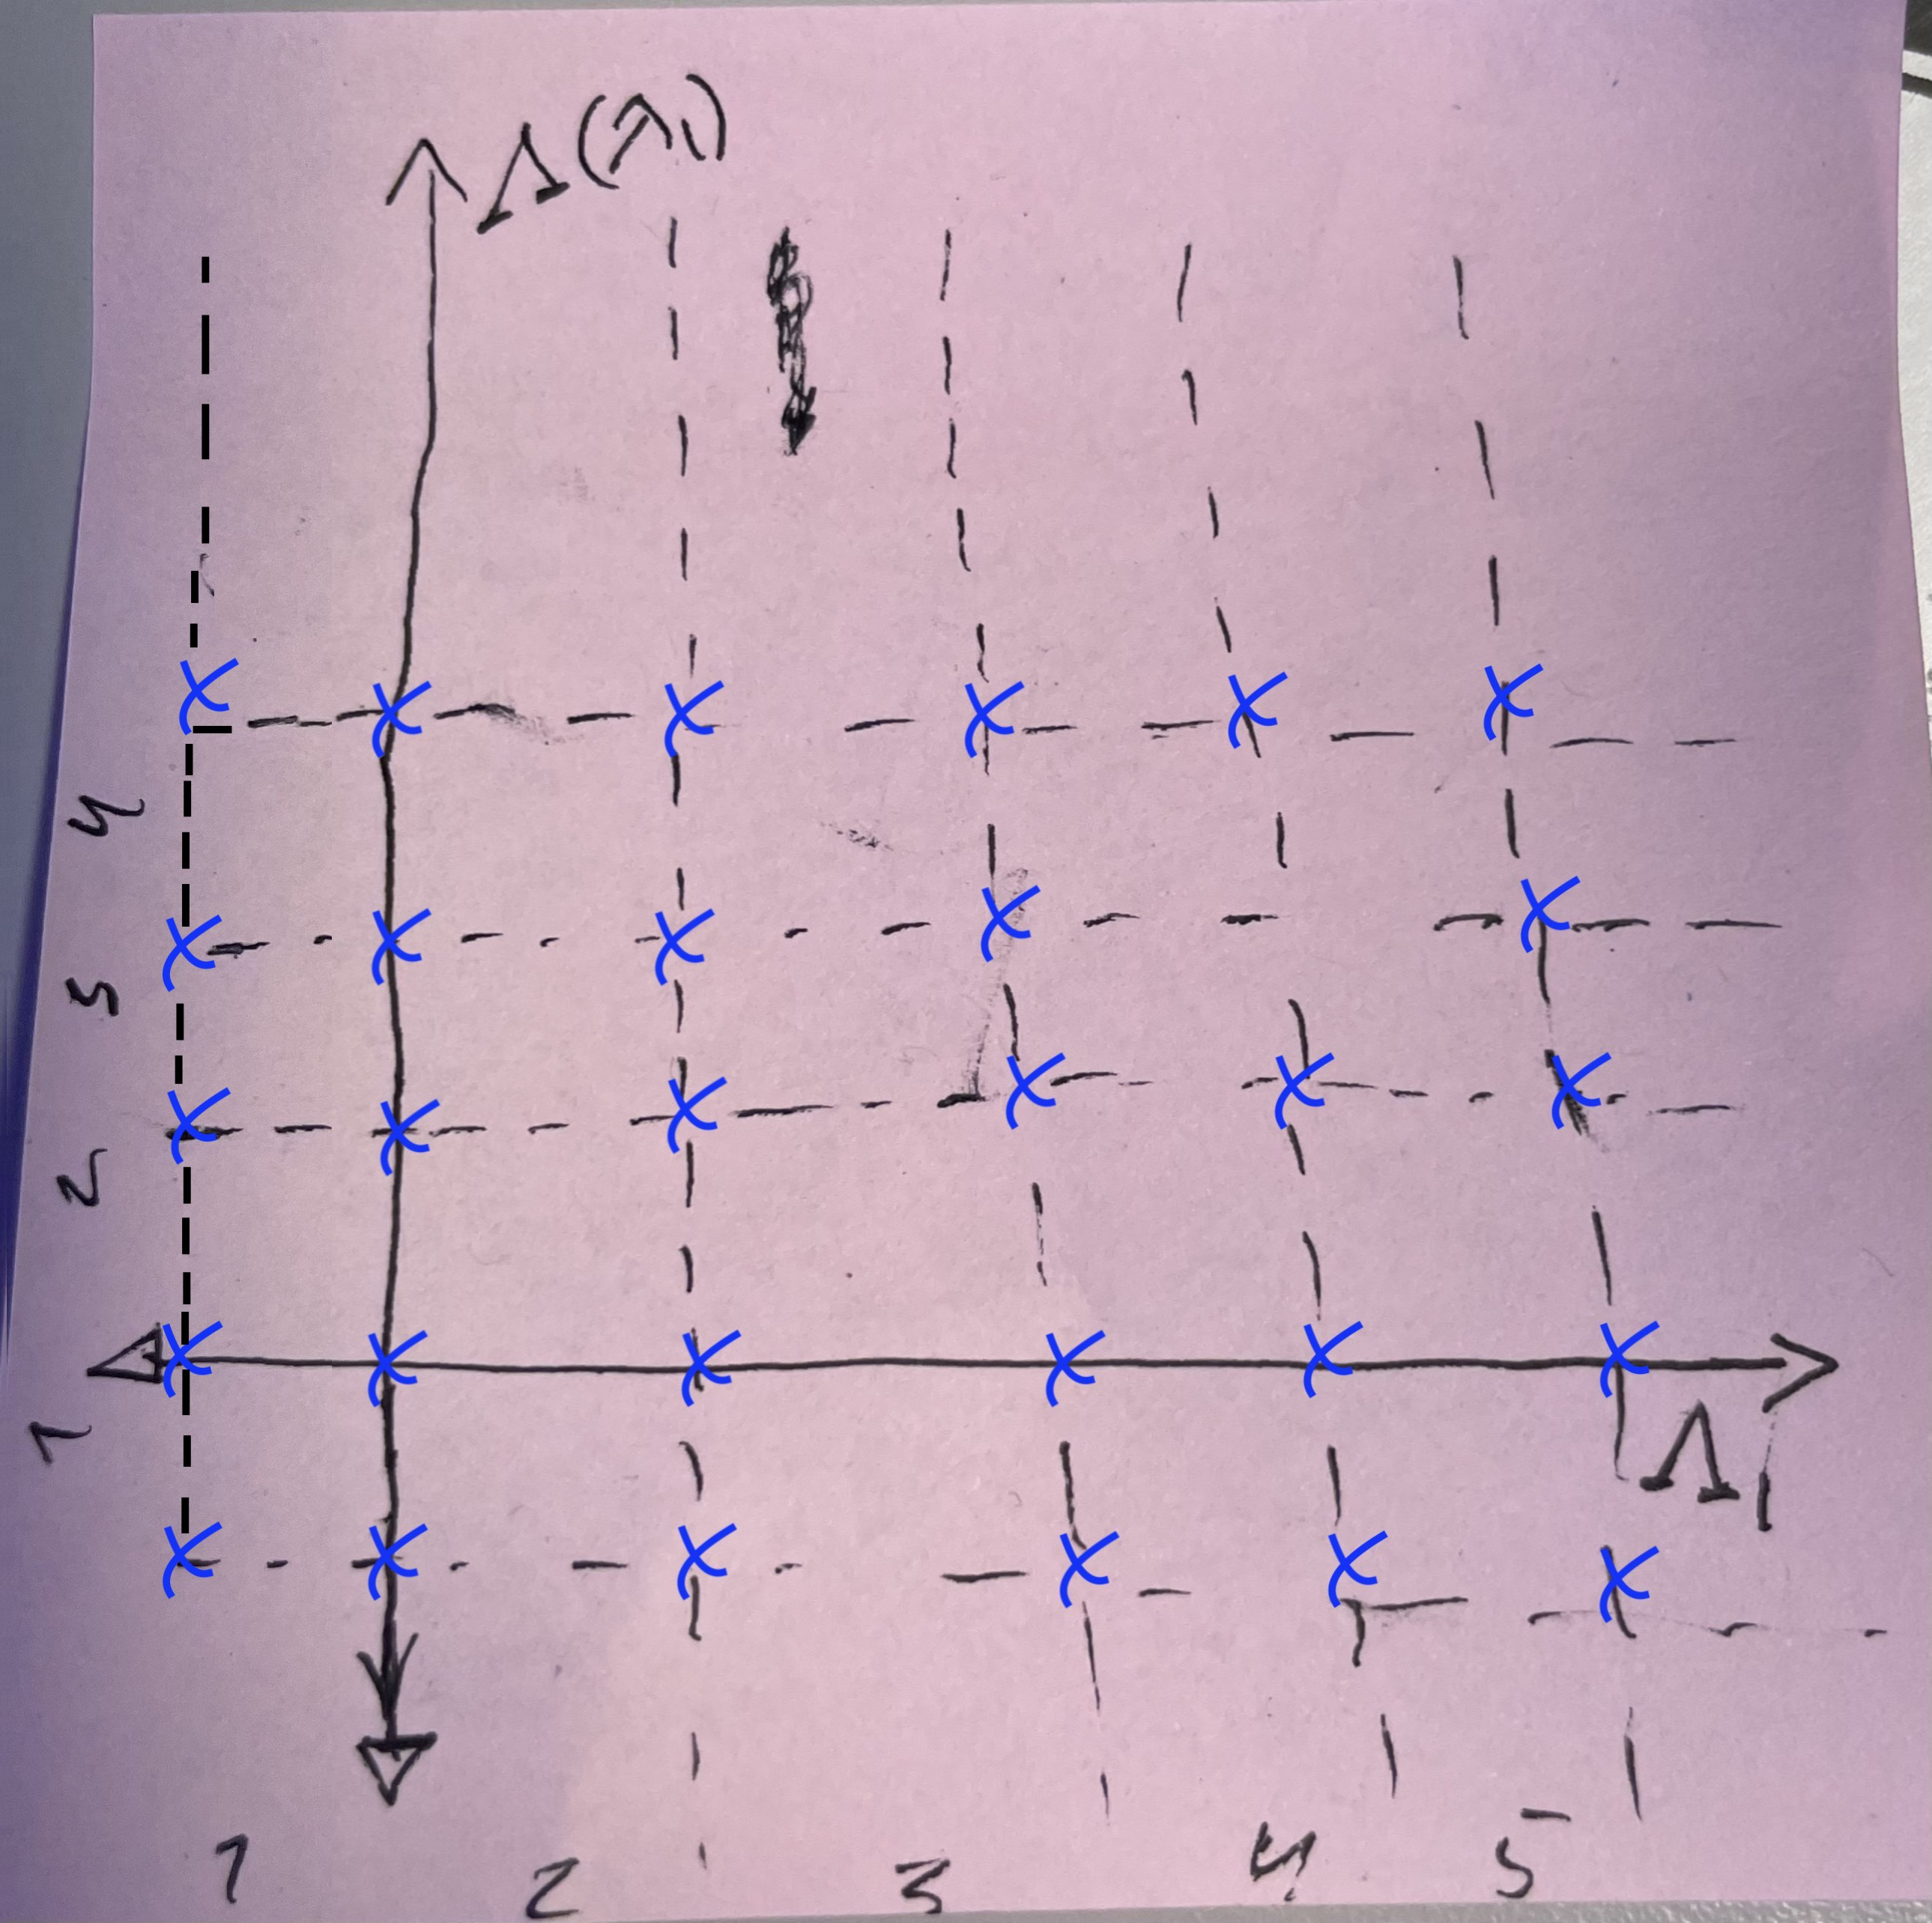
\includegraphics[width=0.9\linewidth]{spec_no_shift.jpg}
        %* Figure 1
        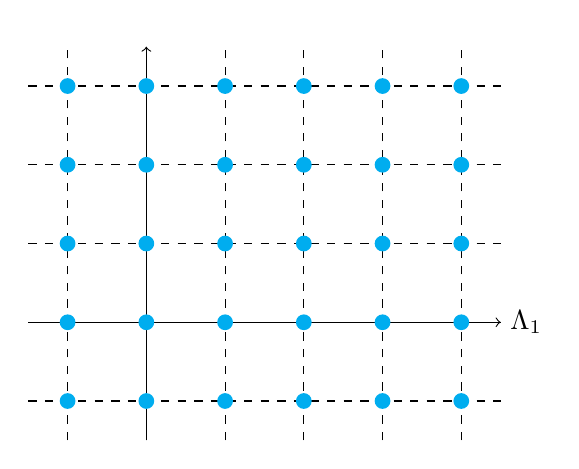
\begin{tikzpicture}
            \foreach \z in {0}{  % Controles whether the axes are inverted or not, 1 = yes, anything else = no
                

\ifnum\z=1
    % Axis lines
    %\draw[->] (-1.5,0) -- (4.5,0) node[above, xshift=2ex] {$\lambfuncGen{\lambda_2}$};
    \draw[->] (-1.5,0) -- (4.5,0) node[right] {$\lambfuncGen{\lambda_2}$};
    \draw[->] (0,-1.5) -- (0,3.5) node[above] {$\Lambda_2$};

    % Dashed lines at each integer in the x direction
    \foreach \x in {-1,...,4}
        \draw[dashed] (\x,-1.5) -- (\x,3.5);

    % Dashed lines at each integer in the y direction
    \foreach \y in {-1,...,3}
        \draw[dashed] (-1.5,\y) -- (4.5,\y);
\else
    % Axis lines
    \draw[->] (-1.5,0) -- (4.5,0) node[right] {$\Lambda_1$};
    \draw[->] (0,-1.5) -- (0,3.5) node[above] {$\lambfunc$};

    % Dashed lines at each integer in the x direction
    \foreach \x in {-1,...,4}
        \draw[dashed] (\x,-1.5) -- (\x,3.5);

    % Dashed lines at each integer in the y direction
    \foreach \y in {-1,...,3}
        \draw[dashed] (-1.5,\y) -- (4.5,\y);
\fi
                % Cyan circles at an integer coordinate with no border
                \foreach \x in {-1,...,4}
                    \foreach \y in {-1,...,3}
                        \fill[cyan] (\x,\y) circle (0.1);
            }
        \end{tikzpicture}
        %* —————————————————
        \caption{Lattice spectra}
        %?  \label{fig:lattice_spectra}
    \end{subfigure}\quad
    \begin{subfigure}{.47\textwidth}
        \centering
        %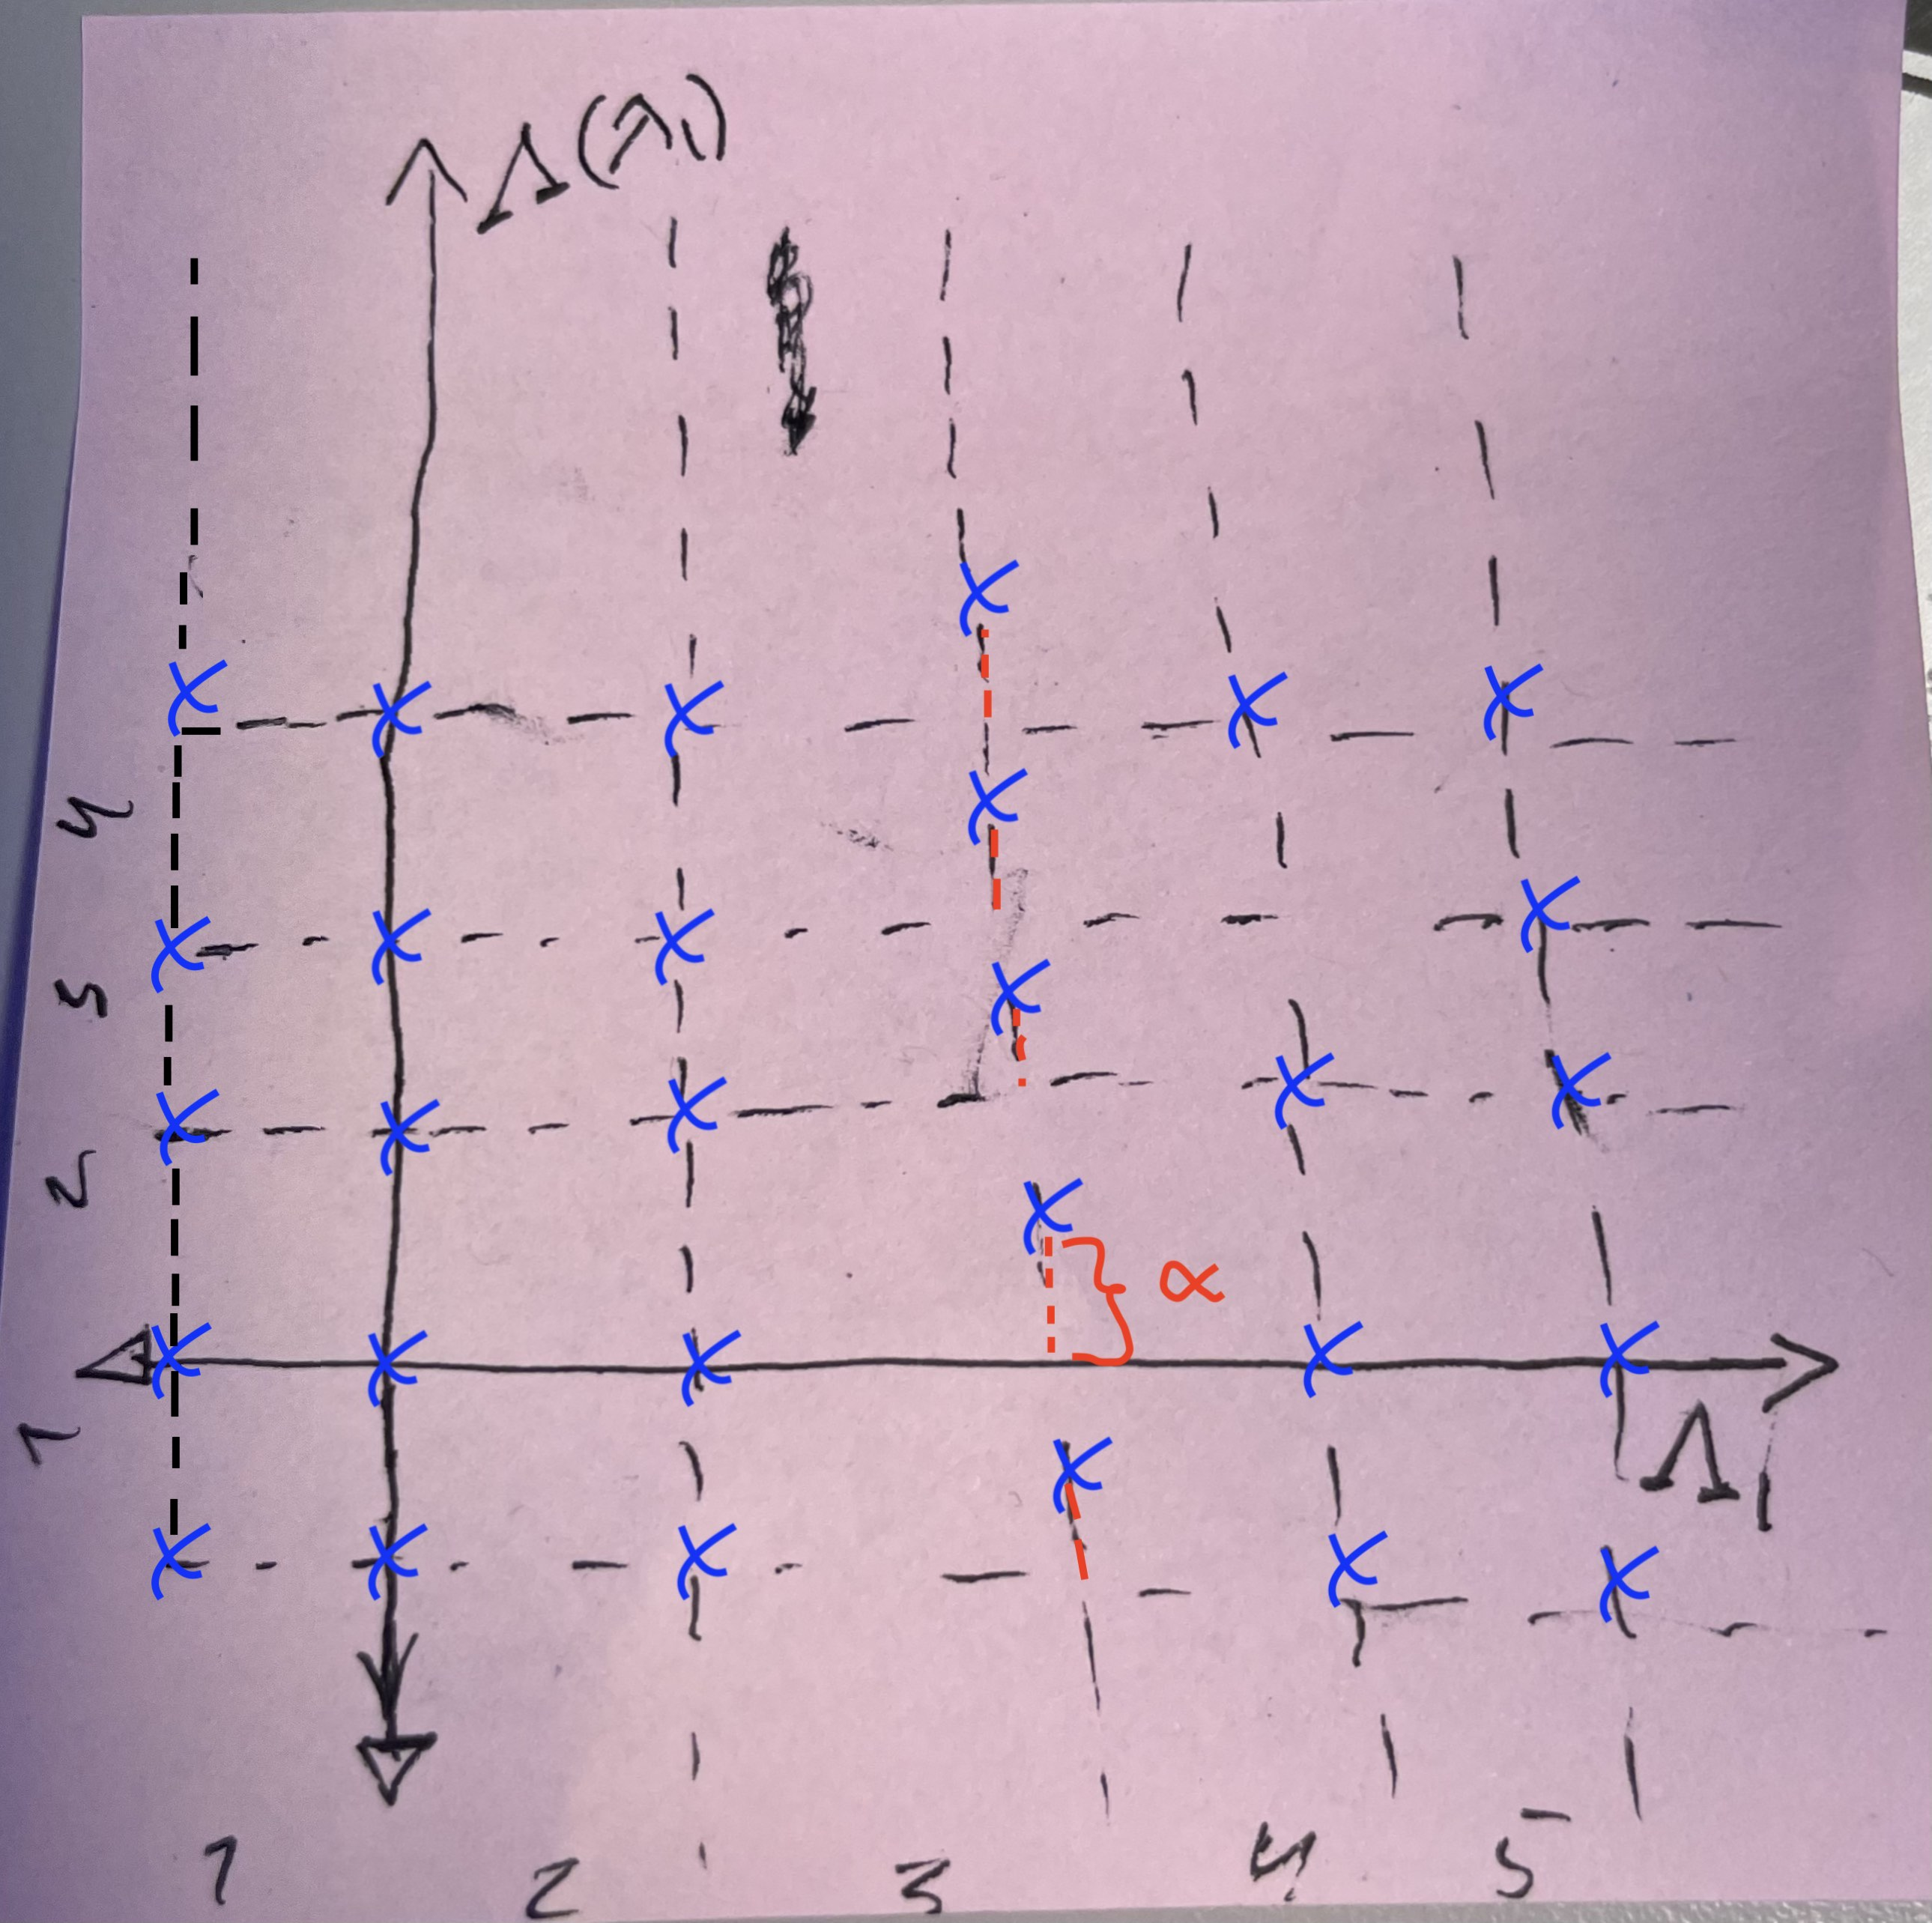
\includegraphics[width=0.9\linewidth]{spec_single_shift.jpg}
        %* Figure 2
        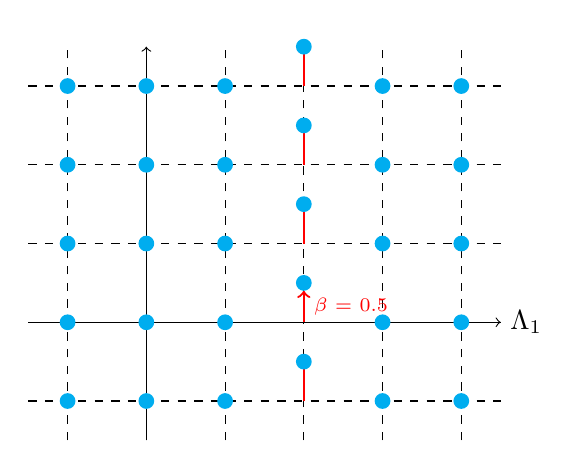
\begin{tikzpicture}
            \foreach \z in {0}{  % Controles whether the axes are inverted or not, 1 = yes, anything else = no
                

\ifnum\z=1
    % Axis lines
    %\draw[->] (-1.5,0) -- (4.5,0) node[above, xshift=2ex] {$\lambfuncGen{\lambda_2}$};
    \draw[->] (-1.5,0) -- (4.5,0) node[right] {$\lambfuncGen{\lambda_2}$};
    \draw[->] (0,-1.5) -- (0,3.5) node[above] {$\Lambda_2$};

    % Dashed lines at each integer in the x direction
    \foreach \x in {-1,...,4}
        \draw[dashed] (\x,-1.5) -- (\x,3.5);

    % Dashed lines at each integer in the y direction
    \foreach \y in {-1,...,3}
        \draw[dashed] (-1.5,\y) -- (4.5,\y);
\else
    % Axis lines
    \draw[->] (-1.5,0) -- (4.5,0) node[right] {$\Lambda_1$};
    \draw[->] (0,-1.5) -- (0,3.5) node[above] {$\lambfunc$};

    % Dashed lines at each integer in the x direction
    \foreach \x in {-1,...,4}
        \draw[dashed] (\x,-1.5) -- (\x,3.5);

    % Dashed lines at each integer in the y direction
    \foreach \y in {-1,...,3}
        \draw[dashed] (-1.5,\y) -- (4.5,\y);
\fi
                % The single shift 
                \def\BetaSingle{0.5}

                % x in the range [-1,1]
                % Cyan circles at an integer coordinate with no border
                \foreach \x in {-1,...,1}
                \foreach \y in {-1,...,3}
                    \fill[cyan] (\x,\y) circle (0.1);  % Cyan circle
                    %\draw[fill=cyan] (\x,\y) circle (0.1);  % Black circle with cyan fill

                % x = 2
                \foreach \x in {2}{
                \foreach \y in {-1,...,3}{
                    \ifnum\y=0
                        \draw[->, thick, red] (\x,\y) -- (\x,\y+\BetaSingle-0.1) node[midway, right] {\scriptsize $\beta$ = \BetaSingle};  % Line indicating the shift amount
                        %\draw[thick, red] (\x,\y) -- (\x,\y+\BetaSingle-0.1) node[midway, right] {\scriptsize $\beta$ = \BetaSingle};  % Line indicating the shift amount
                    \else
                        \draw[thick, red] (\x,\y) -- (\x,\y+\BetaSingle);  % Line indicating the shift amount
                    \fi
                    \fill[cyan] (\x,\y+\BetaSingle) circle (0.1);  % Cyan circles at an integer coordinate with no border
                    %\draw[fill=cyan] (\x,\y+\BetaSingle) circle (0.1);  % Black circle with cyan fill
                }}

                % x in the range [3,4]
                % Cyan circles at an integer coordinate with no border
                \foreach \x in {3,...,4}{
                    \foreach \y in {-1,...,3}{
                        \fill[cyan] (\x,\y) circle (0.1);  % Cyan circle
                        %\draw[fill=cyan] (\x,\y) circle (0.1);  % Black circle with cyan fill
                }}
            }
        \end{tikzpicture}
        %* —————————————————
        \caption{Single shift vertical}
        %?  \label{fig:single_shift_vertical}
    \end{subfigure}\\
    \begin{subfigure}{.47\textwidth}
        \centering
        %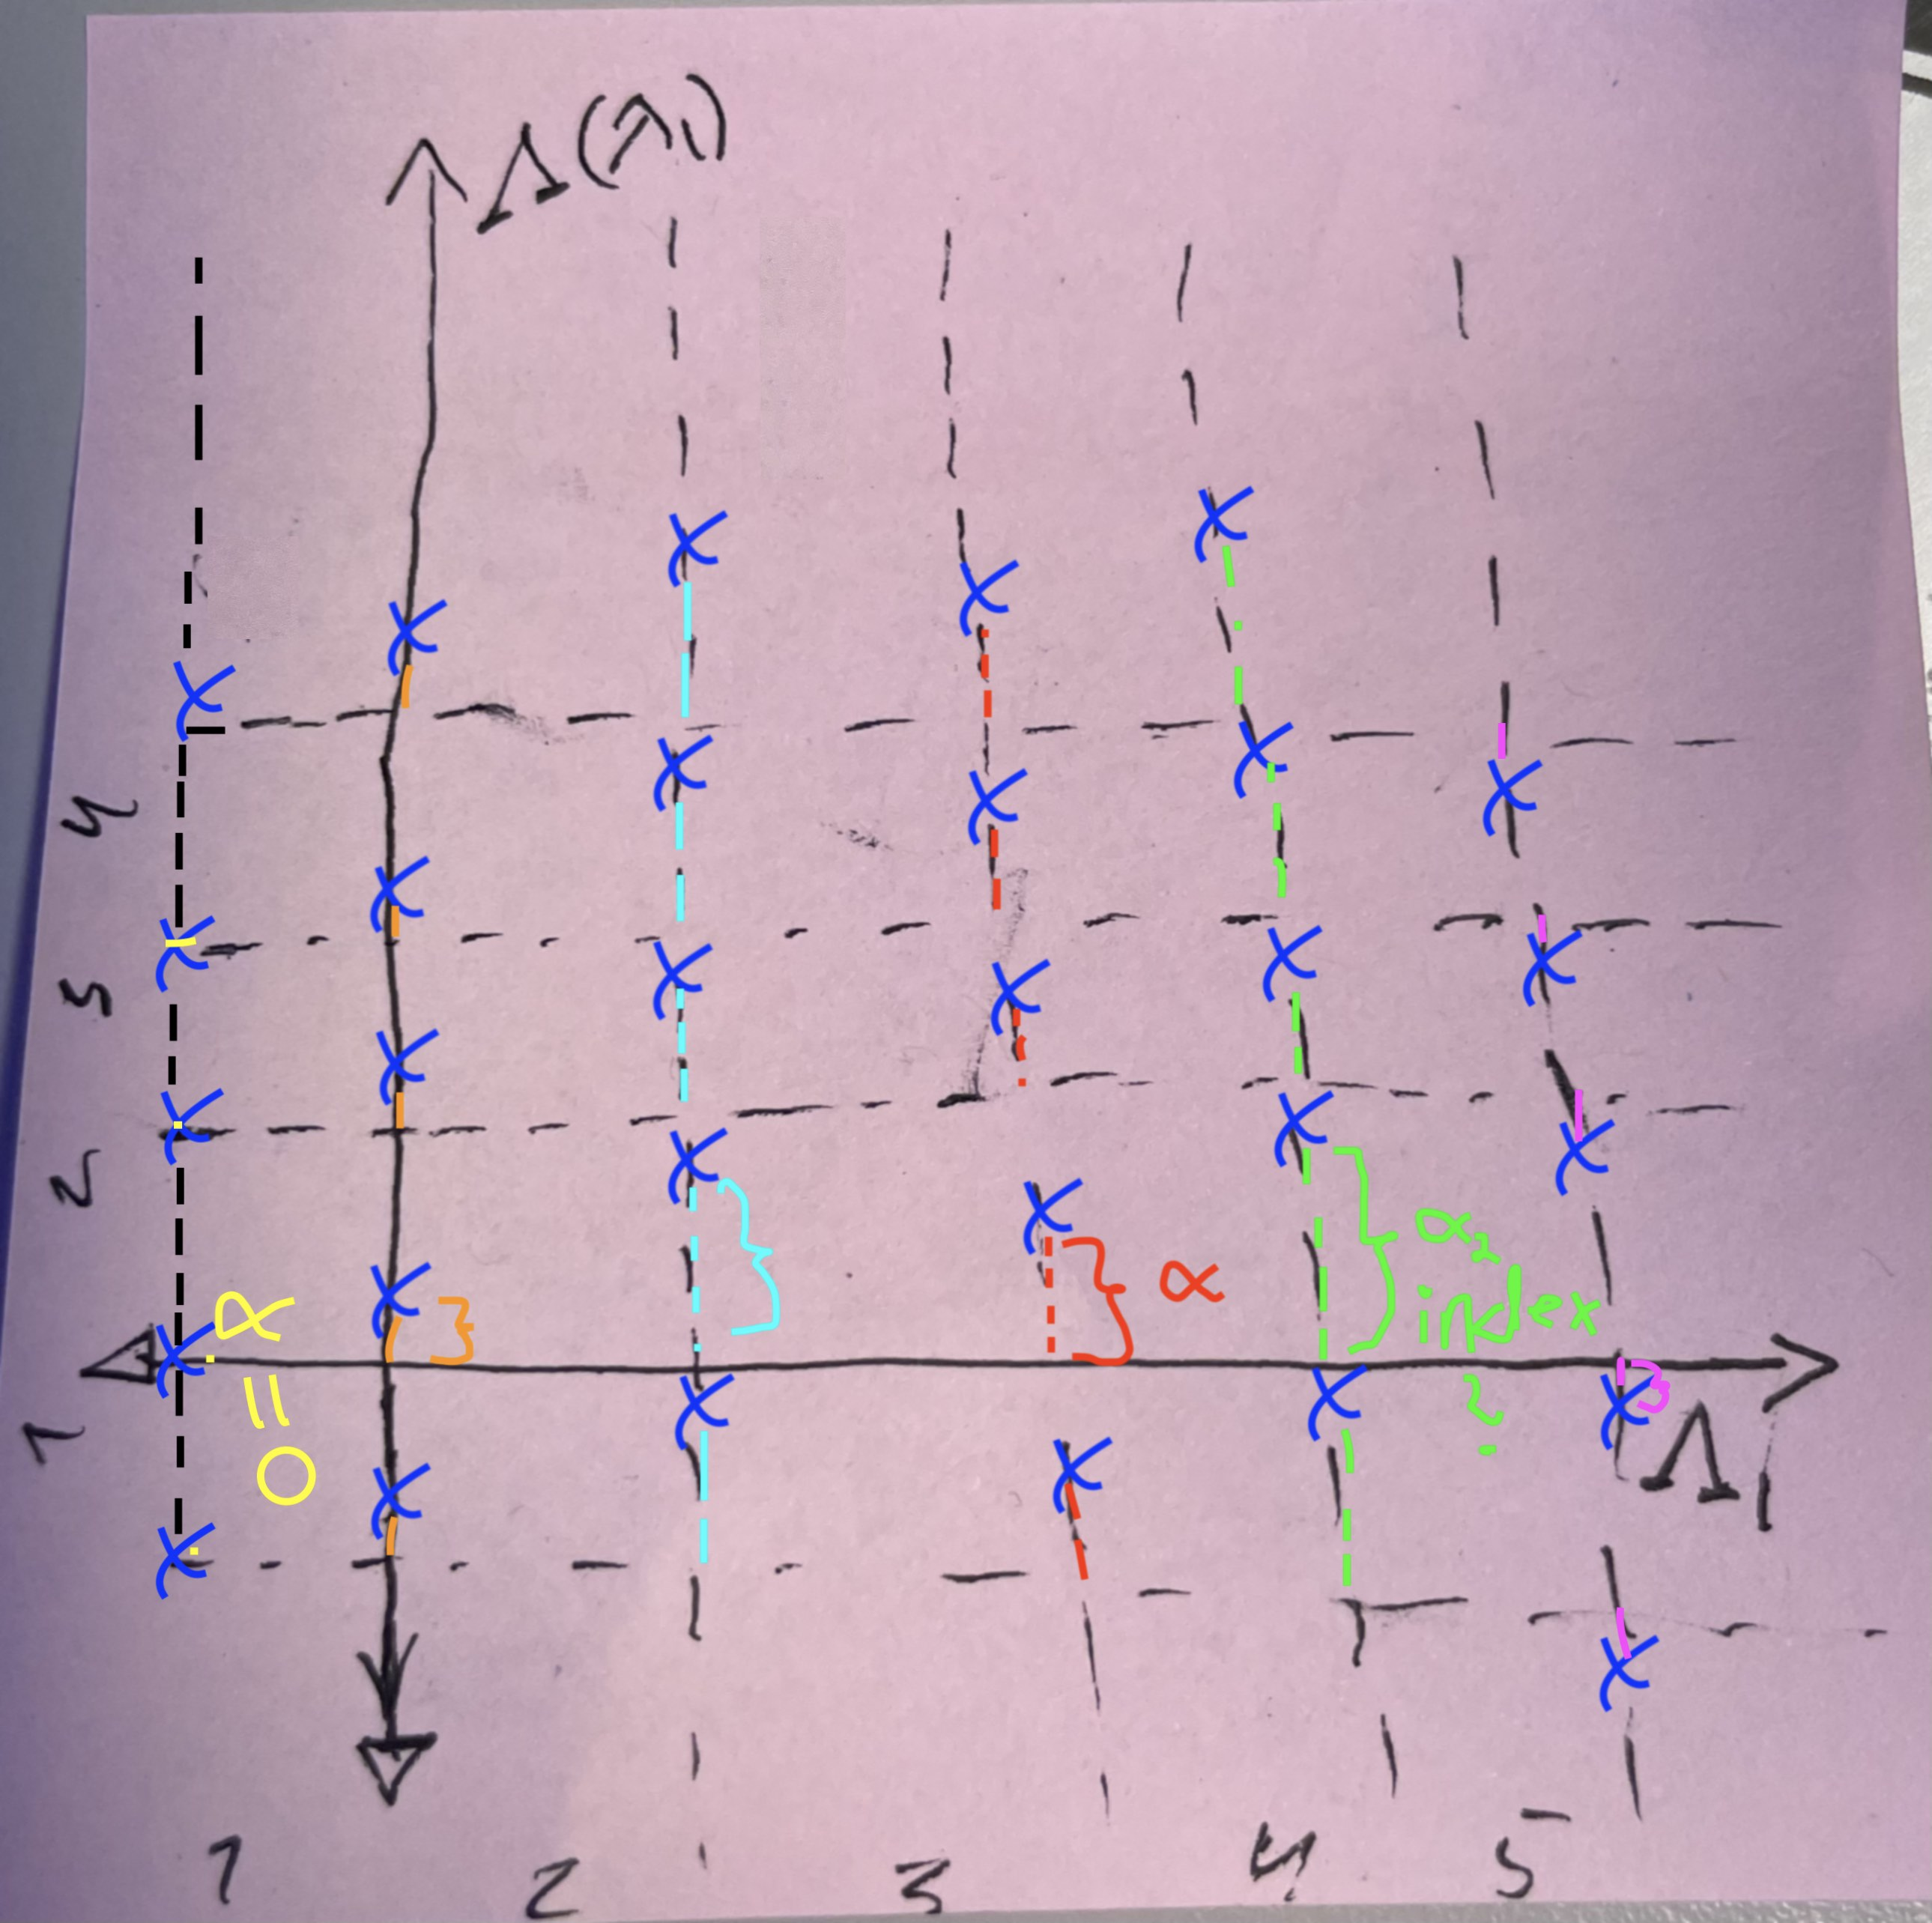
\includegraphics[width=0.9\linewidth]{multiple_shift_left_zero.jpg}
        %* Figure 3
        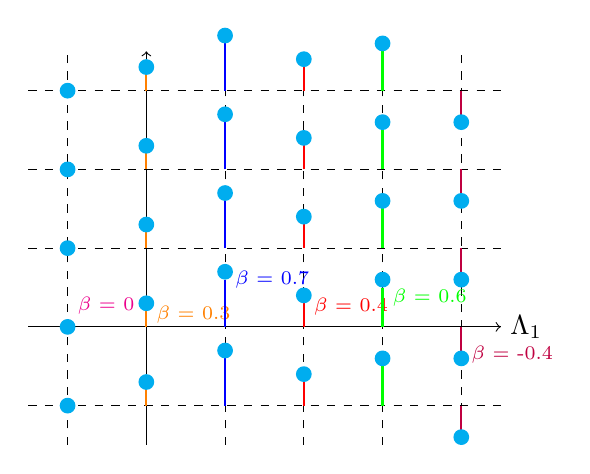
\begin{tikzpicture}
            \foreach \z in {0}{  % Controles whether the axes are inverted or not, 1 = yes, anything else = no
                

\ifnum\z=1
    % Axis lines
    %\draw[->] (-1.5,0) -- (4.5,0) node[above, xshift=2ex] {$\lambfuncGen{\lambda_2}$};
    \draw[->] (-1.5,0) -- (4.5,0) node[right] {$\lambfuncGen{\lambda_2}$};
    \draw[->] (0,-1.5) -- (0,3.5) node[above] {$\Lambda_2$};

    % Dashed lines at each integer in the x direction
    \foreach \x in {-1,...,4}
        \draw[dashed] (\x,-1.5) -- (\x,3.5);

    % Dashed lines at each integer in the y direction
    \foreach \y in {-1,...,3}
        \draw[dashed] (-1.5,\y) -- (4.5,\y);
\else
    % Axis lines
    \draw[->] (-1.5,0) -- (4.5,0) node[right] {$\Lambda_1$};
    \draw[->] (0,-1.5) -- (0,3.5) node[above] {$\lambfunc$};

    % Dashed lines at each integer in the x direction
    \foreach \x in {-1,...,4}
        \draw[dashed] (\x,-1.5) -- (\x,3.5);

    % Dashed lines at each integer in the y direction
    \foreach \y in {-1,...,3}
        \draw[dashed] (-1.5,\y) -- (4.5,\y);
\fi
                % Shift list
                \def\BetaMinOne{0}
                \def\BetaZero{0.3}
                \def\BetaOne{0.7}
                \def\BetaTwo{0.4}
                \def\BetaThree{0.6}
                \def\BetaFour{-0.4}

                % x = -1
                \foreach \x in {-1}{
                \foreach \y in {-1,...,3}{
                    \ifnum\y=0
                    \draw[thick, magenta] (\x,\y) -- (\x,\y+0.05\BetaMinOne) node[midway, above right] {\scriptsize $\beta$ = \BetaMinOne};  % Line indicating the shift amount
                    \else
                    \draw[thick, magenta] (\x,\y) -- (\x,\y+\BetaMinOne);  % Line indicating the shift amount
                    \fi
                    \fill[cyan] (\x,\y+\BetaMinOne) circle (0.1);  % Cyan circles at an integer coordinate with no border
                }}
                % x = 0
                \foreach \x in {0}{
                \foreach \y in {-1,...,3}{
                    \ifnum\y=0
                    %\draw[->, orange] (\x,\y) -- (\x,\y+\BetaZero-0.1) node[near end, right] {\scriptsize $\beta$ = \BetaZero};  % Line indicating the shift amount
                    \draw[thick, orange] (\x,\y) -- (\x,\y+\BetaZero-0.1) node[near end, right] {\scriptsize $\beta$ = \BetaZero};  % Line indicating the shift amount
                    \else
                    \draw[thick, orange] (\x,\y) -- (\x,\y+\BetaZero);  % Line indicating the shift amount
                    \fi
                    \fill[cyan] (\x,\y+\BetaZero) circle (0.1);  % Cyan circles at an integer coordinate with no border
                }}
                % x = 1
                \foreach \x in {1}{
                \foreach \y in {-1,...,3}{
                    \ifnum\y=0
                    %\draw[->, blue] (\x,\y) -- (\x,\y+\BetaOne-0.1) node[at end, right] {\scriptsize $\beta$ = \BetaOne};  % Line indicating the shift amount
                    \draw[thick, blue] (\x,\y) -- (\x,\y+\BetaOne-0.1) node[at end, right] {\scriptsize $\beta$ = \BetaOne};  % Line indicating the shift amount
                    \else
                    \draw[thick, blue] (\x,\y) -- (\x,\y+\BetaOne);  % Line indicating the shift amount
                    \fi
                    \fill[cyan] (\x,\y+\BetaOne) circle (0.1);  % Cyan circles at an integer coordinate with no border
                }}
                % x = 2
                \foreach \x in {2}{
                \foreach \y in {-1,...,3}{
                    \ifnum\y=0
                    %\draw[->, red] (\x,\y) -- (\x,\y+\BetaTwo-0.1) node[very near end, right] {\scriptsize $\beta$ = \BetaTwo};  % Line indicating the shift amount
                    \draw[thick, red] (\x,\y) -- (\x,\y+\BetaTwo-0.1) node[very near end, right] {\scriptsize $\beta$ = \BetaTwo};  % Line indicating the shift amount
                    \else
                    \draw[thick, red] (\x,\y) -- (\x,\y+\BetaTwo);  % Line indicating the shift amount
                    \fi
                    \fill[cyan] (\x,\y+\BetaTwo) circle (0.1);  % Cyan circles at an integer coordinate with no border
                }}
                % x = 3
                \foreach \x in {3}{
                \foreach \y in {-1,...,3}{
                    \ifnum\y=0
                    %\draw[->, green] (\x,\y) -- (\x,\y+\BetaThree-0.1) node[near end, right] {\scriptsize $\beta$ = \BetaThree};  % Line indicating the shift amount
                    \draw[thick, green] (\x,\y) -- (\x,\y+\BetaThree-0.1) node[near end, right] {\scriptsize $\beta$ = \BetaThree};  % Line indicating the shift amount
                    \else
                    \draw[thick, green] (\x,\y) -- (\x,\y+\BetaThree);  % Line indicating the shift amount
                    \fi
                    \fill[cyan] (\x,\y+\BetaThree) circle (0.1);  % Cyan circles at an integer coordinate with no border
                }}
                % x = 4
                \foreach \x in {4}{
                \foreach \y in {-1,...,3}{
                    \ifnum\y=0
                    %\draw[->, purple] (\x,\y) -- (\x,\y+\BetaFour+0.1) node[at end, right, yshift=-0.5mm] {\scriptsize $\beta$ = \BetaFour};  % Line indicating the shift amount
                    \draw[thick, purple] (\x,\y) -- (\x,\y+\BetaFour+0.1) node[at end, right, yshift=-0.5mm] {\scriptsize $\beta$ = \BetaFour};  % Line indicating the shift amount
                    \else
                    \draw[thick, purple] (\x,\y) -- (\x,\y+\BetaFour);  % Line indicating the shift amount
                    \fi
                    \fill[cyan] (\x,\y+\BetaFour) circle (0.1);  % Cyan circles at an integer coordinate with no border
                }}
            }
        \end{tikzpicture}
        %* —————————————————
        \caption{Multiple individual shifts vertical}
        %?  \label{fig:multiple_shift_vertical}
    \end{subfigure}\quad
    \begin{subfigure}{.47\textwidth}
        \centering
        %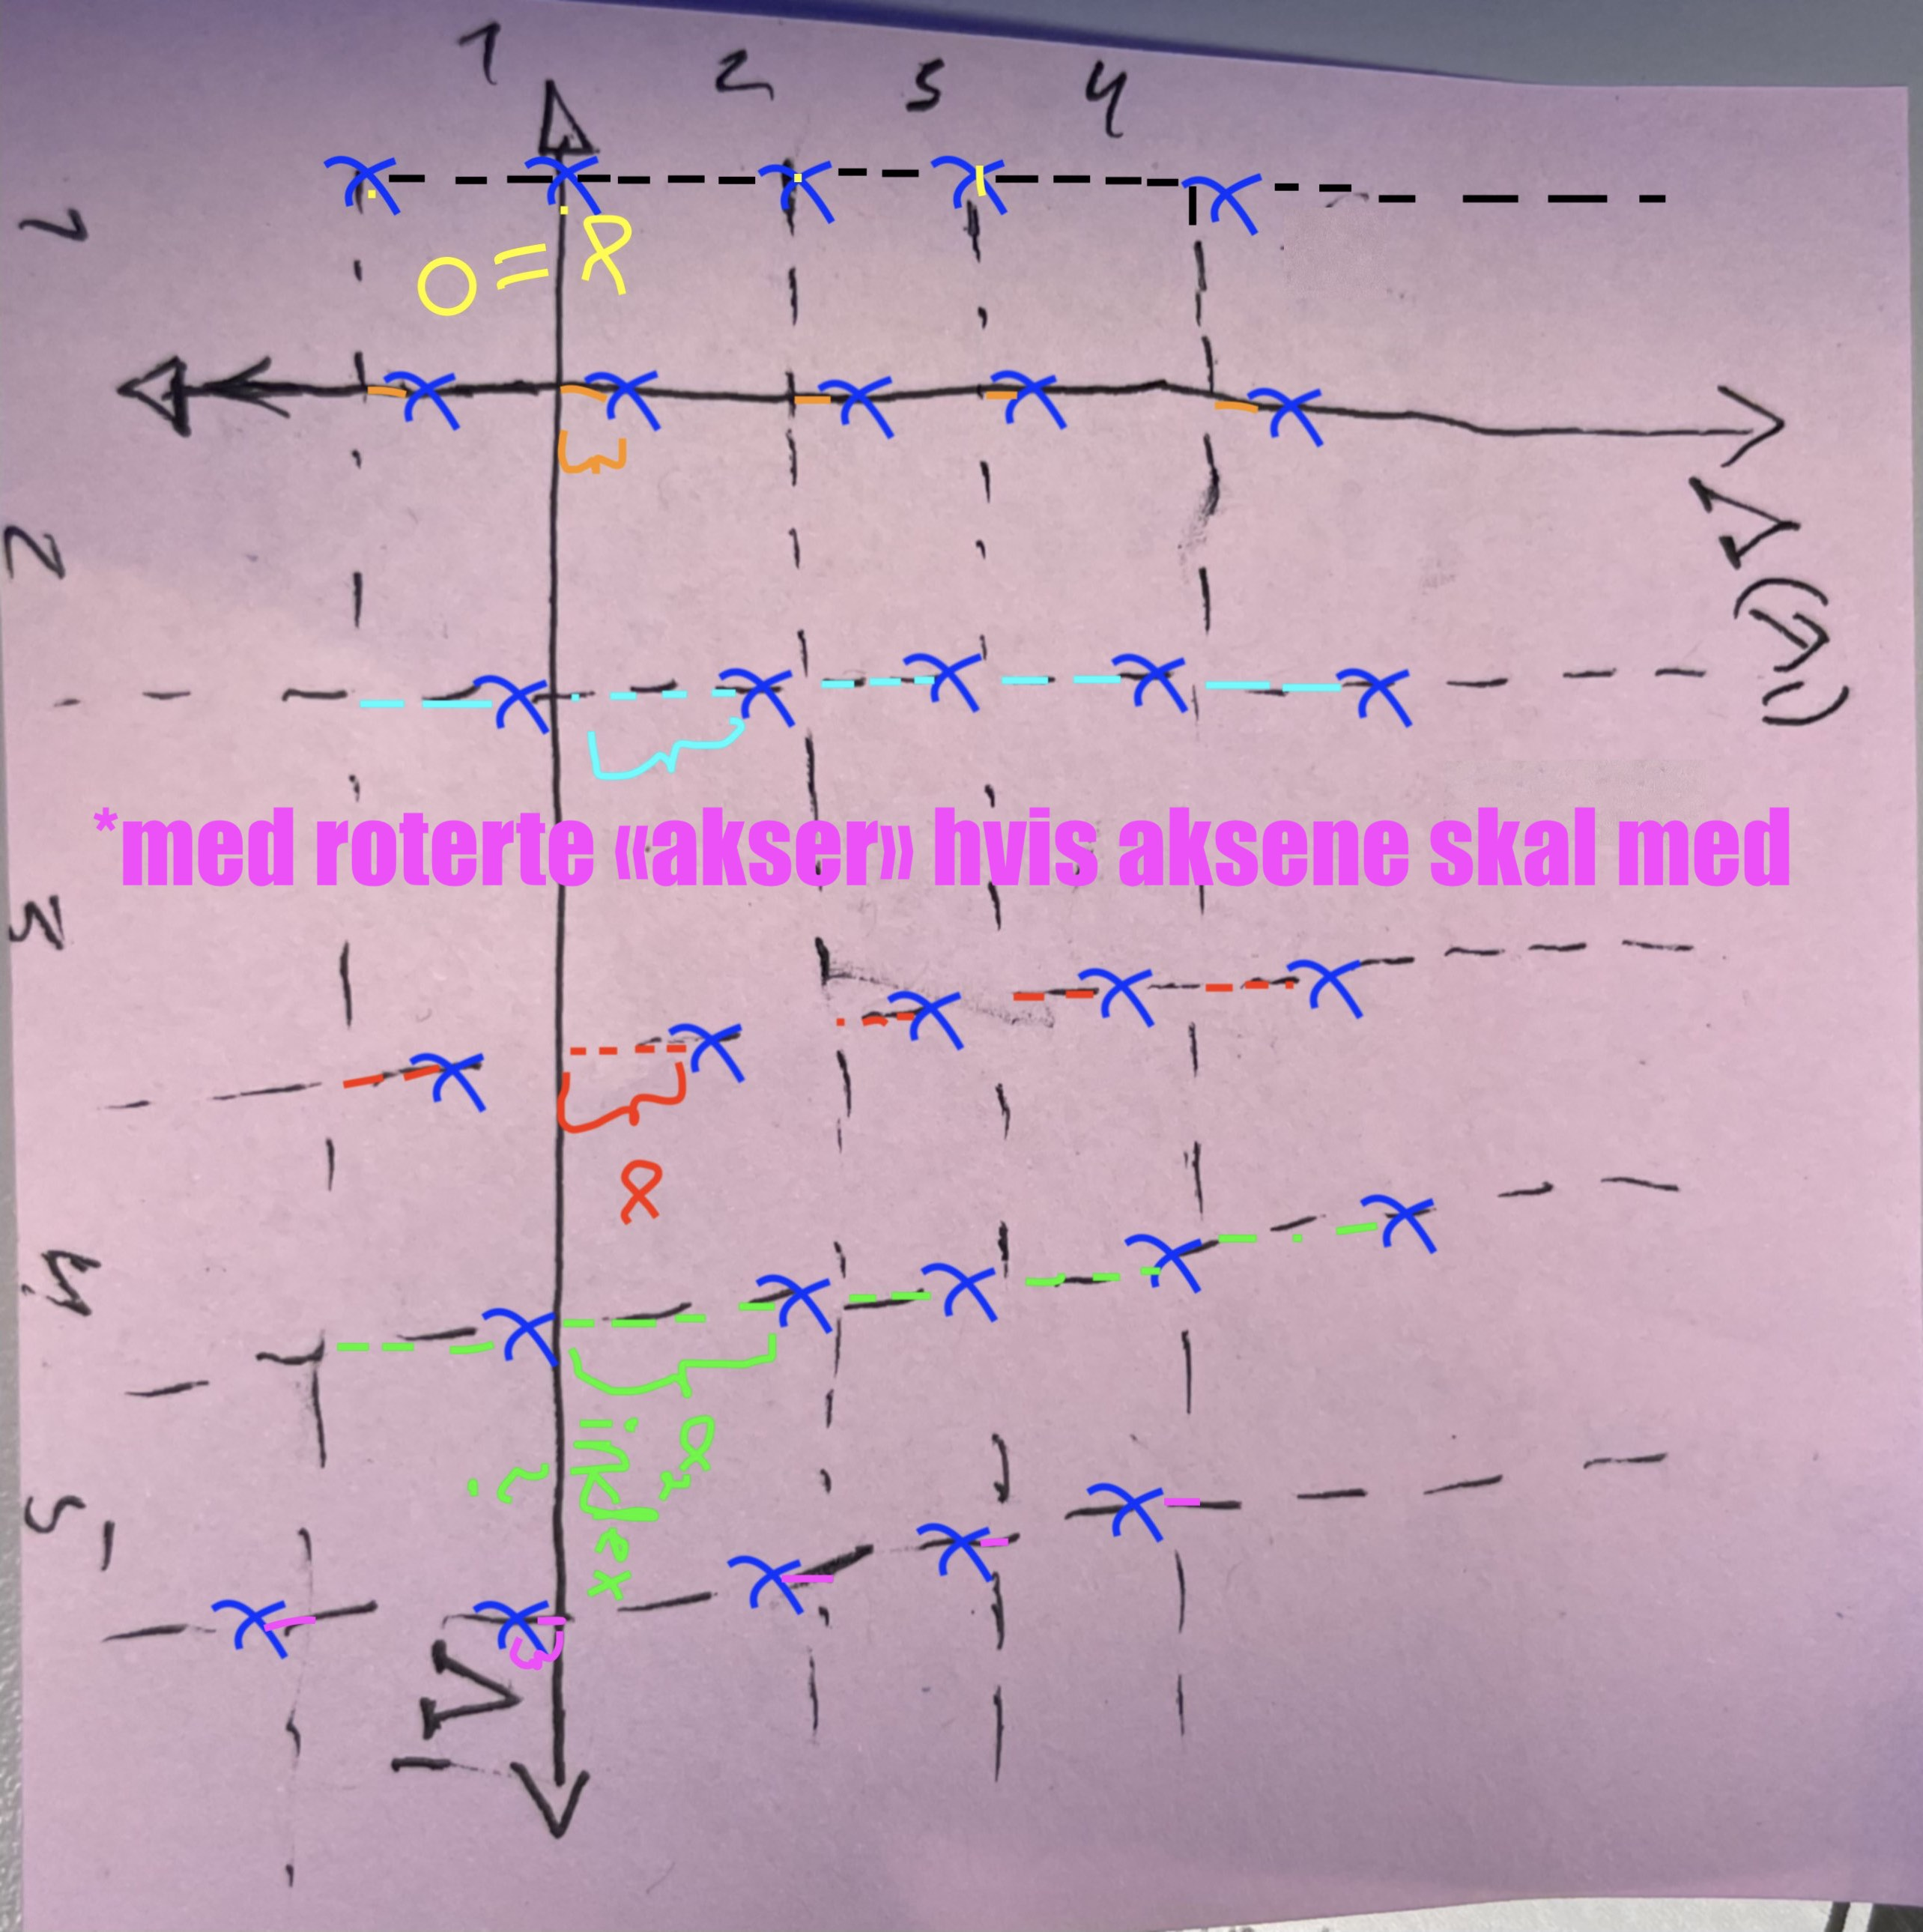
\includegraphics[width=0.9\linewidth]{multiple_shift_left_zero_horizontal.jpg}
        %* Figure 4
        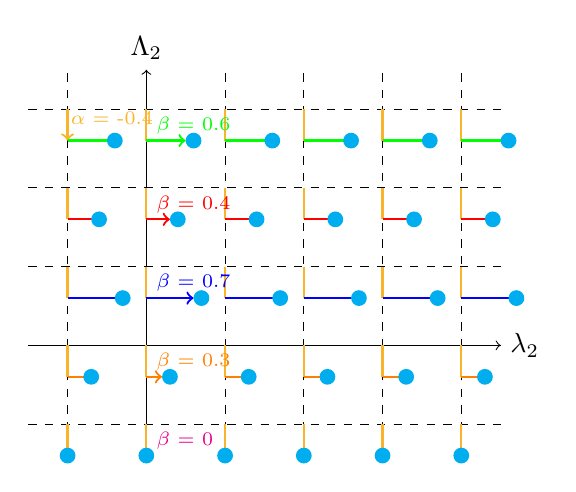
\begin{tikzpicture}
            \foreach \z in {1}{  % Controles whether the axes are inverted or not, 1 = yes, anything else = no
                

\ifnum\z=1
    % Axis lines
    %\draw[->] (-1.5,0) -- (4.5,0) node[above, xshift=2ex] {$\lambfuncGen{\lambda_2}$};
    \draw[->] (-1.5,0) -- (4.5,0) node[right] {$\lambfuncGen{\lambda_2}$};
    \draw[->] (0,-1.5) -- (0,3.5) node[above] {$\Lambda_2$};

    % Dashed lines at each integer in the x direction
    \foreach \x in {-1,...,4}
        \draw[dashed] (\x,-1.5) -- (\x,3.5);

    % Dashed lines at each integer in the y direction
    \foreach \y in {-1,...,3}
        \draw[dashed] (-1.5,\y) -- (4.5,\y);
\else
    % Axis lines
    \draw[->] (-1.5,0) -- (4.5,0) node[right] {$\Lambda_1$};
    \draw[->] (0,-1.5) -- (0,3.5) node[above] {$\lambfunc$};

    % Dashed lines at each integer in the x direction
    \foreach \x in {-1,...,4}
        \draw[dashed] (\x,-1.5) -- (\x,3.5);

    % Dashed lines at each integer in the y direction
    \foreach \y in {-1,...,3}
        \draw[dashed] (-1.5,\y) -- (4.5,\y);
\fi
                % Shift list
                \def\BetaMinOne{0}
                \def\BetaZero{0.3}
                \def\BetaOne{0.7}
                \def\BetaTwo{0.4}
                \def\BetaThree{0.6}
                \def\BetaFour{-0.6}
                \def\AlphaONE{-0.4}

                % The X shift lines at x=0
                \foreach \x in {-1,...,4}{
                \foreach \y in {-1,...,3}{
                    \ifnum\x=-1
                        \ifnum\y=3
                            \draw[->, thick, Dandelion] (\x,\y) -- (\x,\y+\AlphaONE) node[pos=0.3, right, xshift=-0.9mm] {\scriptsize $\alpha$ = \AlphaONE};  % Line indicating the shift amount
                        \else
                            %\draw[->, thick, purple] (\x,\y) -- (\x,\y+\AlphaONE);  % Line indicating the shift amount
                            \draw[thick, Dandelion] (\x,\y) -- (\x,\y+\AlphaONE);  % Line indicating the shift amount
                        \fi
                    \else
                    \draw[thick, Dandelion] (\x,\y) -- (\x,\y+\AlphaONE);  % Line indicating the shift amount
                    \fi
                }}

                % The Y shift
                % y = -1
                \foreach \y in {-1}{
                \foreach \x in {-1,...,4}{
                    \ifnum\x=0
                    % no arrow here. It looks ugly for thick lines
                    \draw[thick, magenta] (\x,\y+\AlphaONE) -- (\x+\BetaMinOne+0.05, \y+\AlphaONE) node[at start, above right, yshift=-0.5mm] {\scriptsize $\beta$ = \BetaMinOne};  % Line indicating the shift amount
                    \else
                    \draw[thick, magenta] (\x,\y+\AlphaONE) -- (\x+\BetaMinOne,\y+\AlphaONE);  % Line indicating the shift amount
                    \fi
                    \fill[cyan] (\x+\BetaMinOne,\y+\AlphaONE) circle (0.1);  % Cyan circles at an integer coordinate with no border
                }}
                % y = 0
                \foreach \y in {0}{
                \foreach \x in {-1,...,4}{
                    \ifnum\x=0
                    \draw[->, thick, orange] (\x,\y+\AlphaONE) -- (\x+\BetaZero-0.1,\y+\AlphaONE) node[at start, above right, yshift=-0.5mm] {\scriptsize $\beta$ = \BetaZero};  % Line indicating the shift amount
                    \else
                    \draw[thick, orange] (\x,\y+\AlphaONE) -- (\x+\BetaZero,\y+\AlphaONE);  % Line indicating the shift amount
                    \fi
                    \fill[cyan] (\x+\BetaZero,\y+\AlphaONE) circle (0.1);  % Cyan circles at an integer coordinate with no border
                }}
                % y = 1
                \foreach \y in {1}{
                \foreach \x in {-1,...,4}{
                    \ifnum\x=0
                    \draw[->, thick, blue] (\x,\y+\AlphaONE) -- (\x+\BetaOne-0.1,\y+\AlphaONE) node[at start, above right, yshift=-0.5mm] {\scriptsize $\beta$ = \BetaOne};  % Line indicating the shift amount
                    \else
                    \draw[thick, blue] (\x,\y+\AlphaONE) -- (\x+\BetaOne,\y+\AlphaONE);  % Line indicating the shift amount
                    \fi
                    \fill[cyan] (\x+\BetaOne,\y+\AlphaONE) circle (0.1);  % Cyan circles at an integer coordinate with no border
                }}
                % y = 2
                \foreach \y in {2}{
                \foreach \x in {-1,...,4}{
                    \ifnum\x=0
                    \draw[->, thick, red] (\x,\y+\AlphaONE) -- (\x+\BetaTwo-0.1,\y+\AlphaONE) node[at start, above right, yshift=-0.5mm] {\scriptsize $\beta$ = \BetaTwo};  % Line indicating the shift amount
                    \else
                    \draw[thick, red] (\x,\y+\AlphaONE) -- (\x+\BetaTwo,\y+\AlphaONE);  % Line indicating the shift amount
                    \fi
                    \fill[cyan] (\x+\BetaTwo,\y+\AlphaONE) circle (0.1);  % Cyan circles at an integer coordinate with no border
                }}
                % y = 3
                \foreach \y in {3}{
                \foreach \x in {-1,...,4}{
                    \ifnum\x=0
                    \draw[->, thick, green] (\x,\y+\AlphaONE) -- (\x+\BetaThree-0.1,\y+\AlphaONE) node[at start, above right, yshift=-0.5mm] {\scriptsize $\beta$ = \BetaThree};  % Line indicating the shift amount
                    \else
                    \draw[thick, green] (\x,\y+\AlphaONE) -- (\x+\BetaThree,\y+\AlphaONE);  % Line indicating the shift amount
                    \fi
                    \fill[cyan] (\x+\BetaThree,\y+\AlphaONE) circle (0.1);  % Cyan circles at an integer coordinate with no border
                }}
            }
        \end{tikzpicture}
        %* —————————————————
        \caption{Multiple individual shifts horizontal}
        %?  \label{fig:multiple_shift_horizontal}
    \end{subfigure}
    %?  \label{fig:spectra_figures}
    % \caption{Illustration of four spectral pairs for $(I^2,\Lambda)$ on a coordinate plane $X\times Y$. Dashed lines highlight the coordinate plane itself, and the cyan circles represent elements from the spectrum. In \cref{fig:lattice_spectra,fig:single_shift_vertical} $\Lambda$ is given by \labelcref{eq:first_construction} and \labelcref{eq:lam_single_shift_vertical} respectivly, where $\beta=0.5$ for the latter. In \cref{fig:multiple_shift_vertical,fig:multiple_shift_horizontal} $\Lambda$ is given by \labelcref{eq:lam_multiple_shift_vertical,eq:lam_multiple_shift_horizontal} respectivly.}
\end{figure}

}  %! End